\documentclass[a4paper,12pt,headsepline]{report}

%----------------- PDF CONFIG ----------------- %
\pdfinfo{    
     /Title (Permissioned Blockchains für B2B - Prototypische Implementierung einer B2B-Anwendung) 
     /Subject   (Permissioned Blockchains)    
     /Author  (Eric Nagel) 
     /Keywords   (Blockchain, B2B)      
}

%TODO: Titel ändern ?
\title{Permissioned Blockchains für B2B - Prototypische Implementierung einer B2B-Anwendung}
\author{Eric Nagel}
\date{09.03.2018}



%----------------- PAKETE INKLUDIEREN ----------------- %

\usepackage{geometry} % Packet für Seitenrandabständex und Einstellung für Seitenränder
\usepackage[ngerman]{babel} % deutsche Silbentrennung

\usepackage{booktabs} %entzerrt die Tabellenzeilen und bietet verschieden dicke Unterteilungslinien
\usepackage{longtable} % Tabellen können sich nicht über mehrere Seiten 
\usepackage{graphicx} % kann LaTeX Grafiken einbinden

\usepackage[utf8]{inputenc}
\usepackage[T1]{fontenc} % Zeichenencoding
\usepackage{lmodern} % typographische Qualität 
\frenchspacing % Schaltet den zusätzlichen Zwischenraum ab
\usepackage{fix-cm}
\usepackage{hyperref} % verwandelt alle Kapitelüberschriften, Verweise aufs Literaturverzeichnis und andere Querverweise in PDF-Hyperlinks
\usepackage{color}
\usepackage{url}
\usepackage{enumitem}

\setitemize{itemsep=-5pt}
\setcounter{secnumdepth}{3}

\usepackage[nottoc]{tocbibind}

% für Listings
\usepackage{listings}
\usepackage{float}
\newfloat{lstfloat}{htbp}{lop}
\floatname{lstfloat}{Listing}
\def\lstfloatautorefname{Listing} % needed for hyperref/auroref
\lstset{numbers=left, numberstyle=\tiny, numbersep=5pt, stepnumber=1, keywordstyle=\color{black}\bfseries\itshape, stringstyle=\ttfamily,showstringspaces=false,basicstyle=\footnotesize,captionpos=b, breaklines=true, postbreak=\mbox{\textcolor{red}{$\hookrightarrow$}\space}}
%\lstset{language=java}

% für Appendex
\usepackage[toc,page]{appendix}

% für Literaturverzeichnis
\usepackage[backend=biber,sorting=none]{biblatex}
\bibliography{literature.bib}

%----------------- FARBEN DEFINIEREN ----------------- %
\definecolor{gray}{gray}{0.97} % Listingsbackground

%----------------- LAYOUT SETZEN ----------------- %
\geometry{left=2cm, right=2cm, top=2.5cm, bottom=2cm}
\linespread {1.25}\selectfont %1.25 da er von Haus aus 1.2 ist und 1,25 * 1,2 = 1,5 isch

%%----------------- INHALT -----------------%
\begin{document}

\pagenumbering{roman} % Seitennummer

 %----------------- KONFIGURATION ----------------- %
\pagestyle{empty} % enthalten keinerlei Kopf oder Fuß 

%----------------- HDA FBI Logo ----------------- %
\begin{figure}[t]
	\centering
	
\includegraphics[width=0.6\textwidth]{images/logo_fbi}
\end{figure}

%----------------- INHALT ----------------- %

\begin{center}
\Large Hochschule Darmstadt \\
\normalsize \textsc{- Fachbereich Informatik -} \\

% Whitespace
\vspace{80 pt}

\Huge Permissioned Blockchains für B2B \\ 
\Large Prototypische Implementierung eines dezentralisierten Wartungsmarktes \\
\normalsize
\vspace{20 pt}

Abschlussarbeit zur Erlangung des akademischen Grades \\ 
Bachelor of Science (B.Sc.) 

\vspace{75 pt}


vorgelegt von \\
\vspace{5 pt}
Eric Nagel \\
Matrikelnummer 740693
\vspace{80 pt}

\begin{tabular}[h]{p{4cm}l l}
	Referent: & Prof. Dr. Andreas Müller \\
	Korreferent: & Björn Bär
\end{tabular}


\end{center}


 %----------------- KONFIGURATION ----------------- %
\pagestyle{empty} % enthalten keinerlei Kopf oder Fuß

%TODO: Abstract eventuell auf 3/4 Seite verlängern
\chapter*{Zusammenfassung} % (fold)
\addcontentsline{toc}{chapter}{Zusammenfassung}
\label{cha:abtract}

Traditionelle B2B-Anwendungen, mit multiplen Unternehmen als Teilnehmer, bringen Probleme bezüglich der Datenhaltung mit sich. Eine Option ist, dass jedes Unternehmen Daten bei sich selber speichert. Dies führt jedoch zu zusätzlichen Aufwand, da Schnittstellen eingerichtet werden müssen, um Geschäftspartnern Zugriff auf relevante Daten zu gewähren. Eine weitere Option ist die Speicherung bei einer zentralen, verwaltenden Instanz. Jeder Geschäftspartner müsste dieser jedoch vertrauen, was die Anwendung unattraktiver macht. Eine Lösung für diese Probleme könnte die Blockchain-Technologie darstellen. Mit ihr ist eine verteilte Datenspeicherung unter nicht vertrauenswürdigen Teilnehmern möglich. Dabei stellt die Blockchain sicher, dass die Daten bei allen Geschäftspartnern synchron sind, und nicht manipuliert oder gelöscht werden können. Die Technologie bringt jedoch auch Schwierigkeiten mit sich, welche für B2B-Anwendungen unerwünscht sind. In Public Blockchains wie Bitcoin und Ethereum äußert sich dies anhand der Skalierbarkeit, Performance und Sicherheit. Permissioned Blockchains, wie Hyperledger Fabric, können diese Probleme zu Teilen lösen. Nichtsdestotrotz sind darauf basierende Anwendungen auf eine bestimmte Performance oder Nutzerzahl limitiert. Auf Grundlage dieser Erkenntnisse wurde ein Prototyp eines automatisierten dezentralen Wartungsmarktes als Proof-of-Concept entwickelt. In diesen können IoT-Geräte Wartungsbedarf erkennen und Wartungsanbieter darauf reagieren.

 
\tableofcontents % Inhaltverzeichnis

\listoffigures % Abbildungen

\listoftables % Tabellen

\renewcommand{\lstlistlistingname}{Listingverzeichnis}
\lstlistoflistings

\pagestyle{plain} % zurueck setzen von roemische seitenanzahl

\pagenumbering{arabic}
\chapter{Einführung und Motivation}
\label{cha:einfuehrung}

Klassische \acs{B2B}-Anwendungen bringen Probleme hinsichtlich der Datenhaltung mit sich. Eine Option ist die Speicherung der Daten jeden Geschäftspartner selbst. Der Datenzugriff untereinander ist dann jedoch, aufgrund von aufwendig einzurichtenden Schnittstellen und uneinheitlichen Datenformaten, erschwert. Eine weitere Möglichkeit ist die Speicherung bei einem zentralen Unternehmen. Dieses hätte jedoch die Kontrolle über die Daten, womit alle anderen Parteien diesem vertrauen müssten. Diese Faktoren machen \acs{B2B}-Anwendungen für die Teilnehmer unattraktiv und erschweren die Entwicklung \cite{KorpelaDigitalSupplyChain2017}\cite{WustyouneedBlockchain2017}.

Um diese Probleme zu lösen, wird ein Prototyp einer dezentralen \acs{B2B}-Applikation, basierend auf der Blockchain-Technologie, entwickelt. Sie erlaubt es, dezentrale Systeme aufzubauen, in welchen sich die Parteien nicht vertrauen. Alle Daten würden bei jedem Teilnehmer des Blockchain-Netzwerks (im Folgenden nur noch Netzwerk genannt) gespeichert werden. Trotzdem sind diese nicht lösch- oder manipulierbar, alle Transaktionen sind lückenlos nachvollziehbar und es besteht ein gemeinsamer Konsens über den Datenbestand \cite{CrosbyBlockChainTechnologyBitcoin2016}.

Bekannte Blockchain-Implementationen, wie Bitcoin oder Ethereum, bringen jedoch Probleme für den \acs{B2B}-Bereich mit sich. So sind alle Daten öffentlich einsehbar, der Transaktionsdurchsatz ist gering und die Konsensmechanismen sind unter bestimmten Umständen unsicher und resultieren in hohen Energieverbrauch \cite{Gramolidangerprivateblockchains2016}\cite{NakamotoBitcoinPeertoPeerElectronic2008}\cite{EthereumTeamEthereumWhitePaper2017}. 

Ziel dieser Arbeit ist es, die Probleme der Blockchain-Technologie für den \acs{B2B}-Bereich zu analysieren und basierend auf den Ergebnissen eine dezentrale \acs{B2B}-Anwendung als Proof-of-Concept zu entwickeln. Dazu werden zunächst die grundlegenden Konzepte der Blockchain-Technologie erläutert, um ein besseres Verständnis für die Vor- und Nachteile dieser zu erhalten. Anschließend werden die Probleme für \acs{B2B}-Anwendungen anhand der Anforderungen an diese genauer betrachtet und analysiert. Daraufhin erfolgt die Beschreibung der Anwendungsentwicklung. Zuletzt wird ein Fazit zur Lösung der Probleme und des entwickelten Systems gezogen.

\chapter{Grundlagen}
\label{cha:grundlagen}
Zum Verstehen der Diskussion der Probleme der Blockchain-Technologie ist es notwendig, die grundlegenden Konzepte dieser zu verstehen. Weiterhin müssen allgemeine Anforderungen an B2B-Anwendungen erfasst werden, anhand welchen die Diskussion erfolgt.

\section{Blockchain}

\subsection{Funktionsweise}
Die Funktionsweise der Blockchain wird in dieser Arbeit hauptsächlich am Beispiel von Bitcoin erklärt. Als erste Blockchain-Anwendung \cite{ZhengBlockchainChallengesOpportunities2017} und aufgrund der überschaubaren Komplexität liefert es die Grundlage für die Funktionsweise der Technologie. Andere Implementationen, wie Ethereum oder Ripple, funktionieren nach dem gleichen Prinzip.

\subsubsection{Allgemein}
Wenn der Begriff ``Die Blockchain'' auftaucht, ist damit meistens die Blockchain-Technologie gemeint. Es gibt nicht nur eine global bestehende Blockchain und auch nicht nur eine Implementation der Technologie, was beispielsweise anhand von Bitcoin und Ethereum ersichtlich ist.

Allgemein kann die Blockchain als Datenstruktur bezeichnet werden, welche verteilt, nicht lösch- und manipulierbar gespeichert werden kann. Weiterhin verifizieren jegliche Teilnehmer am Netzwerk ausgeführte Transaktionen, wodurch ein gemeinsamer Konsens über den Datenbestand besteht \cite{CrosbyBlockChainTechnologyBitcoin2016}.

In einer Blockchain werden Transaktionen in Blöcken gespeichert. Dabei handelt es sich um Operationen, welche Daten erstellen und manipulieren. Aus diesen lässt sich letztendlich der aktuelle Datenbestand ermitteln. So erfolgt beispielsweise bei Bitcoin keine Speicherung des aktuellen Guthabens der Teilnehmer. Es wird nur aus allen bestehenden Transaktionen berechnet \cite[S.~85]{AntonopoulosMasteringbitcoin2015}. Die Daten, welche letztendlich bestehen, können beispielsweise Geldtransferinformationen (Bitcoin), Smart Contracts (Ethereum, selbst ausführende Verträge mit selbst erstellter Programmlogik, siehe \ref{subsec:use-cases}), simple Dokumente oder Informationen sein \cite{EthereumTeamEthereumWhitePaper2017}\cite{NakamotoBitcoinPeertoPeerElectronic2008}\cite{HyperledgerFabricTeamHyperledgerWhitepaper2016}. Die Blöcke setzen sich aus den Transaktionen sowie den Block Header zusammen, welcher verschiedene Metadaten, wie zum Beispiel den kombinierten Hash\footnote{Hash: Ergebnis einer Operation, welche Daten in eine Zeichenfolge fester Länge umwandelt \cite[S.~\Rn{7}]{SwanBlockchainblueprintnew2015}.} aller Transaktionen, enthält \cite[S.~160-161]{AntonopoulosMasteringbitcoin2015}.

Die Blöcke sind miteinander verkettet. Jeder Block Header enthält den Hash  des vorherigen Block Headers (siehe Abb. \ref{fig:block-chain}). Dies ist ein wichtiges Feature zum Schutz der Blockchain vor Angriffen. Wenn ein Angreifer die Transaktionen eines Blocks zu seinen Gunsten verändern würde, würde sich der Hash des Block Headers ändern. Dieser müsste dann im darauffolgenden Block Header stehen, wodurch sich allerdings auch der Hash dieses Blocks ändert. Letztendlich müssten alle nachfolgenden Blöcke manipuliert werden, um eine gültige Blockchain zu erhalten \cite{NakamotoBitcoinPeertoPeerElectronic2008}. Diese Manipulation wird durch verschiedene Verfahren erschwert, welche genauer in den Kapiteln \ref{subsec:konsens} und \ref{subsec:immutability} erklärt werden.

\begin{figure}[!htbp]
  \centering
	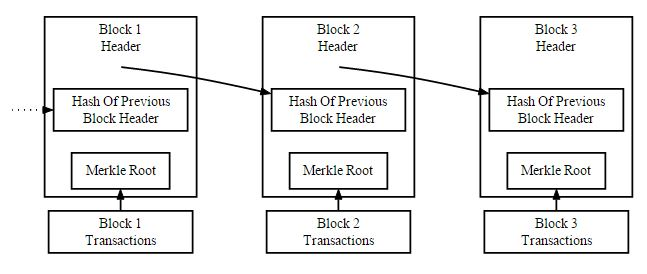
\includegraphics[width=0.85\textwidth,angle=0]{images/block-chain}
 	\caption{Verkettung von Blöcken durch Block Header Hashes \cite{RosicWhatHashingHood2017}.}
	\label{fig:block-chain}
\end{figure}

Die Blockchain ist verteilt gespeichert. Jeder Teilnehmer hat die Möglichkeit Sie auf seinen Rechner zu speichern. Somit besteht keine zentrale Instanz, welche die Kontrolle über die Daten hat. Weiterhin gibt es keinen Single Point of Failure\footnote{Single Point of Failure: Komponente eines Systems, dessen Ausfall den Ausfall des gesamten Systems bewirkt \cite{KshetriCanBlockchainStrengthen2017}.} \cite{KshetriCanBlockchainStrengthen2017}.

\label{subsec:konsens}
\subsubsection{Konsensmechanismen}
Aufgrund der verteilten Datenhaltung muss es Verfahren geben, um die Daten synchron und auf einen Stand, auf welchen sich alle Teilnehmer geeinigt haben, zu halten. Dazu gibt es die sogenannten Konsensmechanismen, welche gleichzeitig die Manipulierbarkeit der Daten verhindern. Bevor diese erklärt werden können, muss zunächst genauer auf die Funktion des Netzwerks eingegangen werden.

\paragraph{Funktion des Netzwerks}
Wenn ein Teilnehmer eine Transaktion ausführt, wird diese, vorausgesetzt dass sie valide ist (genauer im nächsten Absatz erklärt), an alle Nodes\footnote{Node: Teilnehmer eines Blockchain-Netzwerks, welche die Blockchain speichern. Auch Peers genannt.} im Netzwerk weitergeleitet und im Transaktionspool aufgenommen. Dieser enthält alle noch nicht in Blöcken vorkommenden Transaktionen. Diese werden in einen neuen Block aufgenommen, während jede Node mit der Erstellung von diesem beschäftigt ist. Dies wird durch verschiedene Konsensmechanismen realisiert. Bei Bitcoin und Ethereum findet der \acl{PoW} (\acs{PoW}) Anwendung (weiter unten genauer unter erklärt). Sobald eine Node einen Block erstellt, wird dieser im Netzwerk verteilt. Jede Node hängt ihn an ihre lokale Blockchain an und beginnt mit der Erstellung des nächsten Blocks \cite[S.~200 ff.]{AntonopoulosMasteringbitcoin2015}.

Damit eine Transaktion valide ist, muss sie bestimmte Voraussetzungen erfüllen. So muss sie unter anderem mit dem Private Key des Senders signiert sein. Mittels seines Public Keys kann überprüft werden, ob wirklich er der Sender der Nachricht ist und ob die Transaktion manipuliert wurde. Dieses Verfahren wird auch in der Abbildung \ref{fig:key-signing} visualisiert. Das Signieren trägt zur Sicherheit der Blockchain bei, da ein Angreifer dadurch keine Transaktionen eines Nutzers manipulieren oder in seinem Namen ausführen kann. In Bitcoin ist eine weitere Kondition, dass der Transaktionsersteller die zu sendenden Bitcoins besitzt \cite[S.~18]{AntonopoulosMasteringbitcoin2015}. In Systemen wie Ethereum und Hyperledger Fabric, in welchen eigene Programmlogik abgebildet werden kann, können weitere Konditionen festgelegt werden. So muss beispielsweise ein Teilnehmer die nötigen Rechte haben um eine Transaktion auszuführen (siehe \ref{acl}) \cite{HyperledgerComposerTeamAccessControlLanguage}.

\begin{figure}[!htbp]
	\centering
	  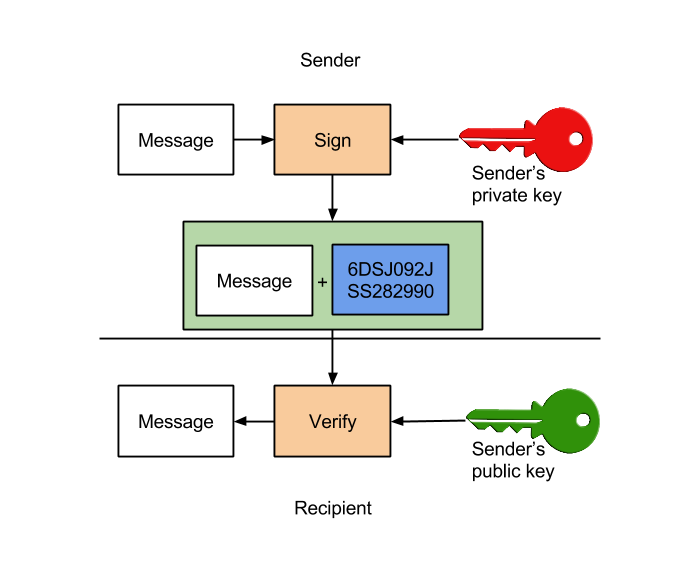
\includegraphics[width=0.4\textwidth,angle=0]{images/key-signing}
	  \caption{Signieren und Verifizieren von Nachrichten. Der Sender signiert die Nachricht mit seinem Private Key und der Empfänger kann diese mit den Public Key des Senders verifizieren \cite{WikimediaCommonsPublickeysigning2006}.}
	  \label{fig:key-signing}
\end{figure}
	
\paragraph{Proof-of-Work}
Der \acs{PoW} ist nur einer der zur Verfügung stehenden Konsensmechanismen (siehe Kapitel \ref{sec:eval-konsens}). Er bedarf jedoch genauerer Erklärung, da er in aktuellen Blockchain-Implementationen vorwiegend genutzt wird. Der \acs{PoW} ist eine Art Rätsel, welches mit der Rechenleistung von Nodes gelöst werden muss, um einen Block zu erschaffen (das sogenannte \textit{Mining}). Genauer gesagt, muss für einen Block ein Hash gefunden werden, welcher einen bestimmten Wert unterschreitet. Um unterschiedliche Hashwerte für gleich bleibende Blöcke zu erhalten, gibt es im Block Header eine Nonce\footnote{Nonce: Eine Nummer, welche genau einmal für einen bestimmten Zweck genutzt wird \cite{MargaretNonceDefinition}.}, welche verändert wird \cite{NakamotoBitcoinPeertoPeerElectronic2008}. Alle Nodes im Netzwerk ändern diese so lange, bis ein gültiger Hash gefunden wird. Desto kleiner der zu findende Hash ist, desto höher ist die Schwierigkeit. Für Sicherheitszwecke ist es nötig, dass die Blockerstellung eine gewisse Zeit benötigt. Um wachsender Rechenleistung und Teilnehmerzahl entgegenzuwirken und somit diese Zeit zu garantieren, kann die Schwierigkeit angepasst werden. Dies wird genauer im Kapitel \ref{sec:scalability-eval} erläutert. Damit die Nodes eine Motivation haben, Rechenleistung für das Erstellen von Blöcken zu nutzen, erhalten sie bei Erbringung des \acs{PoW} eine Belohnung sowie die Transaktionsgebühren in Form von Kryptowährung. In Verbindung mit den Mining sind auch Mining Pools zu erwähnen. Dabei handelt es sich um einen Zusammenschluss von Minern, welche gemeinsam probieren den \acs{PoW} zu erbringen. Gelingt dies, wird die Belohnung zwischen allen Teilnehmern im Pool geteilt.  \cite{NakamotoBitcoinPeertoPeerElectronic2008} \cite{EthereumTeamEthereumWhitePaper2017}. 

\paragraph{Forking}
Um vollständig zu verstehen, wie der \acs{PoW} funktioniert, muss das Forking erklärt werden. Wenn eine Node einen \acs{PoW} erbringt, also einen Block erstellt, wird dieser an alle anderen Nodes weitergeleitet. Im Bitcoin-Netzwerk dauert es bei einer maximalen Blockgröße von 1 MB \cite{SchererPerformanceScalabilityBlockchain2017}, zwischen 6 und 20 Sekunden, bis ein Block mindestens 90 \% aller Nodes erreicht hat \cite{BitcoinStatsBitcoinPropagationData}. Dies stimmt auch mit dem Paper von Decker und Wattenhofer überein, wo eine durchschnittliche Zeit von 12,6 Sekunden angegeben wird, bis ein Block 95 \% aller Nodes erreicht \cite{DeckerInformationpropagationbitcoin2013}. In dieser Zeit kann es vorkommen, dass eine weitere Node einen Block erstellt. Auch dieser wird im Netzwerk verteilt, wodurch zwei Versionen der Blockchain existieren: Eine endet mit Block A und die andere mit Block B. Dies ist der sogenannte Fork. Das Netzwerk muss sich nun darauf einigen, welche der beiden Versionen beibehalten werden soll. Deshalb gilt: Die Blockchain, in welche mehr Arbeit eingeflossen ist, ist die gültige. Im Falle von Bitcoin wäre dies die längere Blockchain. Die Nodes probieren an den zuerst erhaltenen Block (A oder B) einen neuen anzuhängen. Gelingt dies, ist eine der beiden Blockchains länger als die andere. Diese wird dann von allen Nodes als die richtige akzeptiert. Dieser Vorgang wird auch in den Abbildungen \ref{fig:fork_1} bis \ref{fig:fork_4} dargestellt. Theoretisch ist es möglich, dass ein Fork über mehrere Blöcke besteht. Die Wahrscheinlichkeit dafür ist jedoch gering, da mehrmals nacheinander mindestens zwei Nodes zur ungefähr gleichen Zeit einen Block erstellen müssen. Auch zu erwähnen ist, dass in einem Fork-Branch weitere Forks entstehen können. Diese Forks sind der Grund, warum Transaktionen erst als bestätigt gelten, sobald sie in einem Block stehen, welcher eine gewisse Anzahl an Nachfolgern hat. Denn erst dann ist die Sicherheit gegeben, dass die Transaktion nicht in einem Branch vorhanden ist, welcher eventuell verworfen wird \cite[S.~211 ff.]{AntonopoulosMasteringbitcoin2015}. Wie genau der \acs{PoW} das Netzwerk absichert, wird im Kapitel \ref{subsec:immutability} erklärt.

\begin{figure}[!htbp]
  \centering
    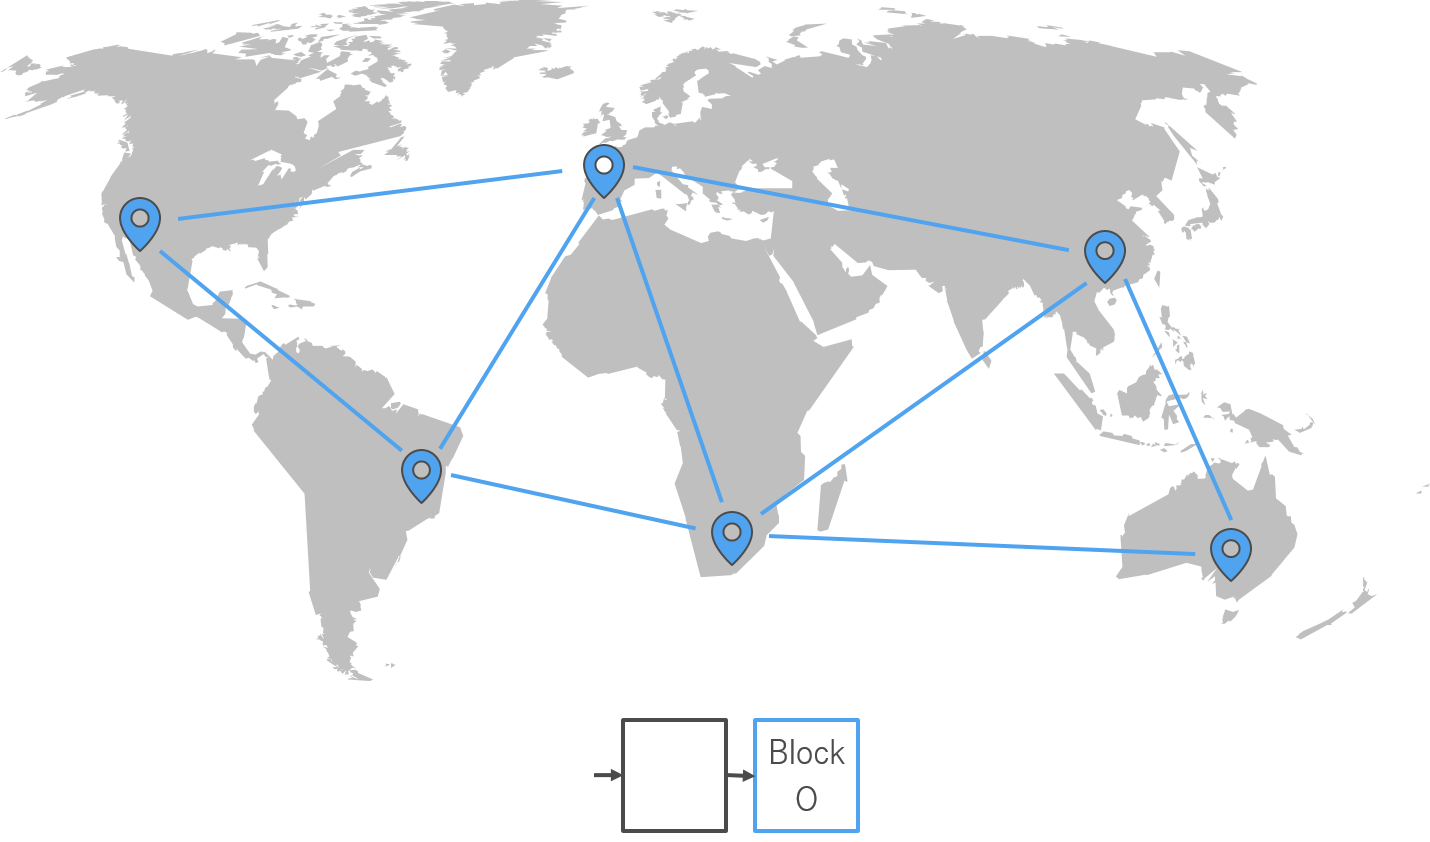
\includegraphics[width=0.95\textwidth,angle=0]{images/fork_1}
 	\caption{Fork-Visualisierung - Vor dem Fork besitzen alle Nodes Block O als letzten Block \cite[S.~200 ff.]{AntonopoulosMasteringbitcoin2015}.}
	\label{fig:fork_1}
\end{figure}

\begin{figure}[!htbp]
  \centering
	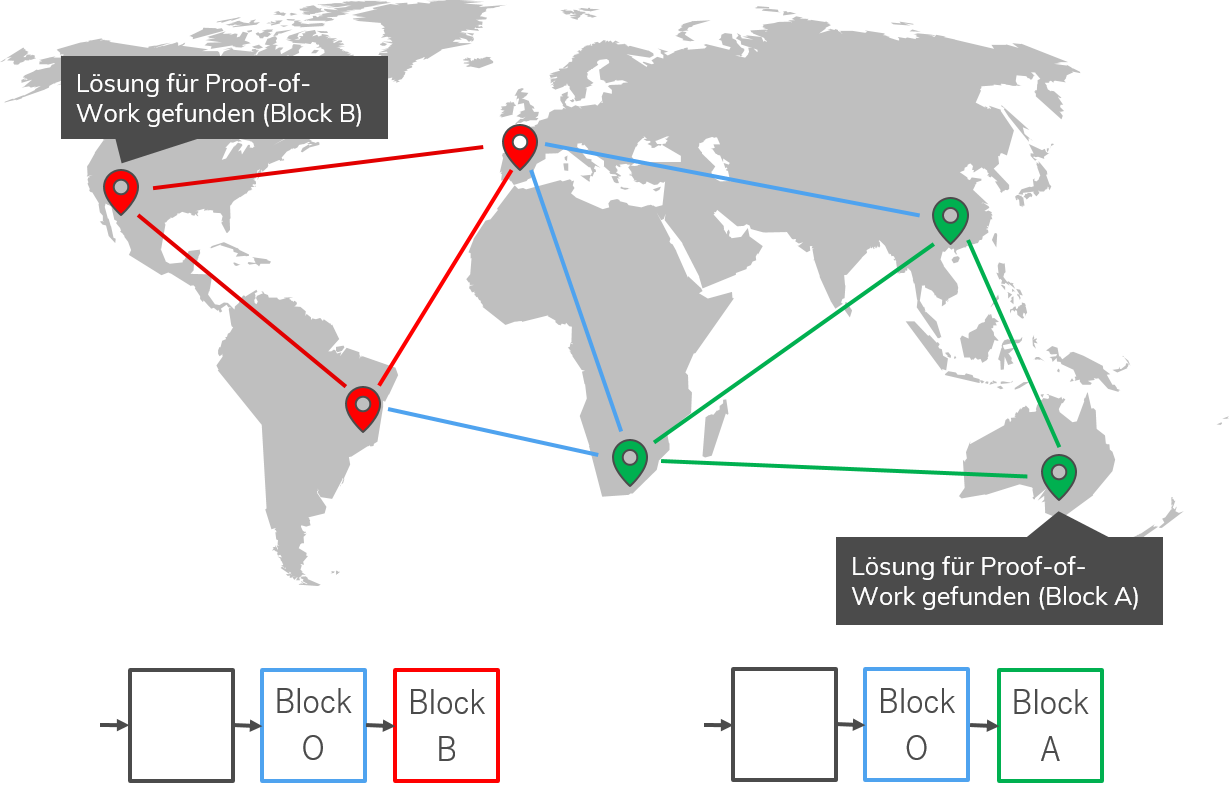
\includegraphics[width=0.95\textwidth,angle=0]{images/fork_2}
 	\caption{Fork-Visualisierung - zwei Nodes finden zur ungefähr gleichen Zeit einen Block und verbreiten ihn im Netzwerk, wodurch zwei Versionen der Blockchain bestehen \cite[S.~200 ff.]{AntonopoulosMasteringbitcoin2015}.}
	\label{fig:fork_2}
\end{figure}

\begin{figure}[!htbp]
  \centering
	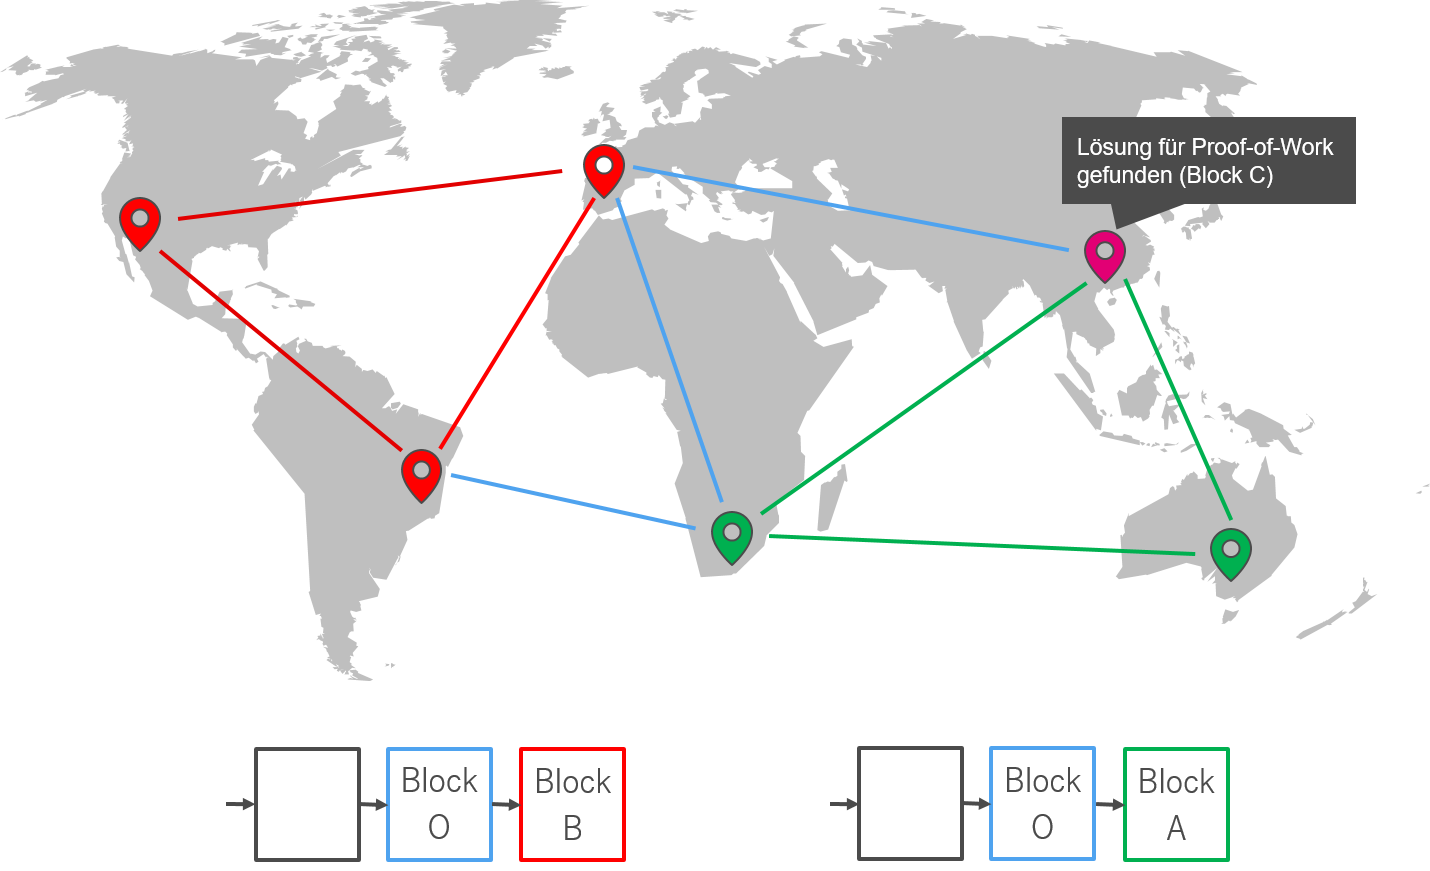
\includegraphics[width=0.95\textwidth,angle=0]{images/fork_3}
 	\caption{Fork-Visualisierung - Eine Node, welche Block A zuerst erhalten hat, hängt daran einen neuen Block C an \cite[S.~200 ff.]{AntonopoulosMasteringbitcoin2015}.}
	\label{fig:fork_3}
\end{figure}

\begin{figure}[!htbp]
  \centering
	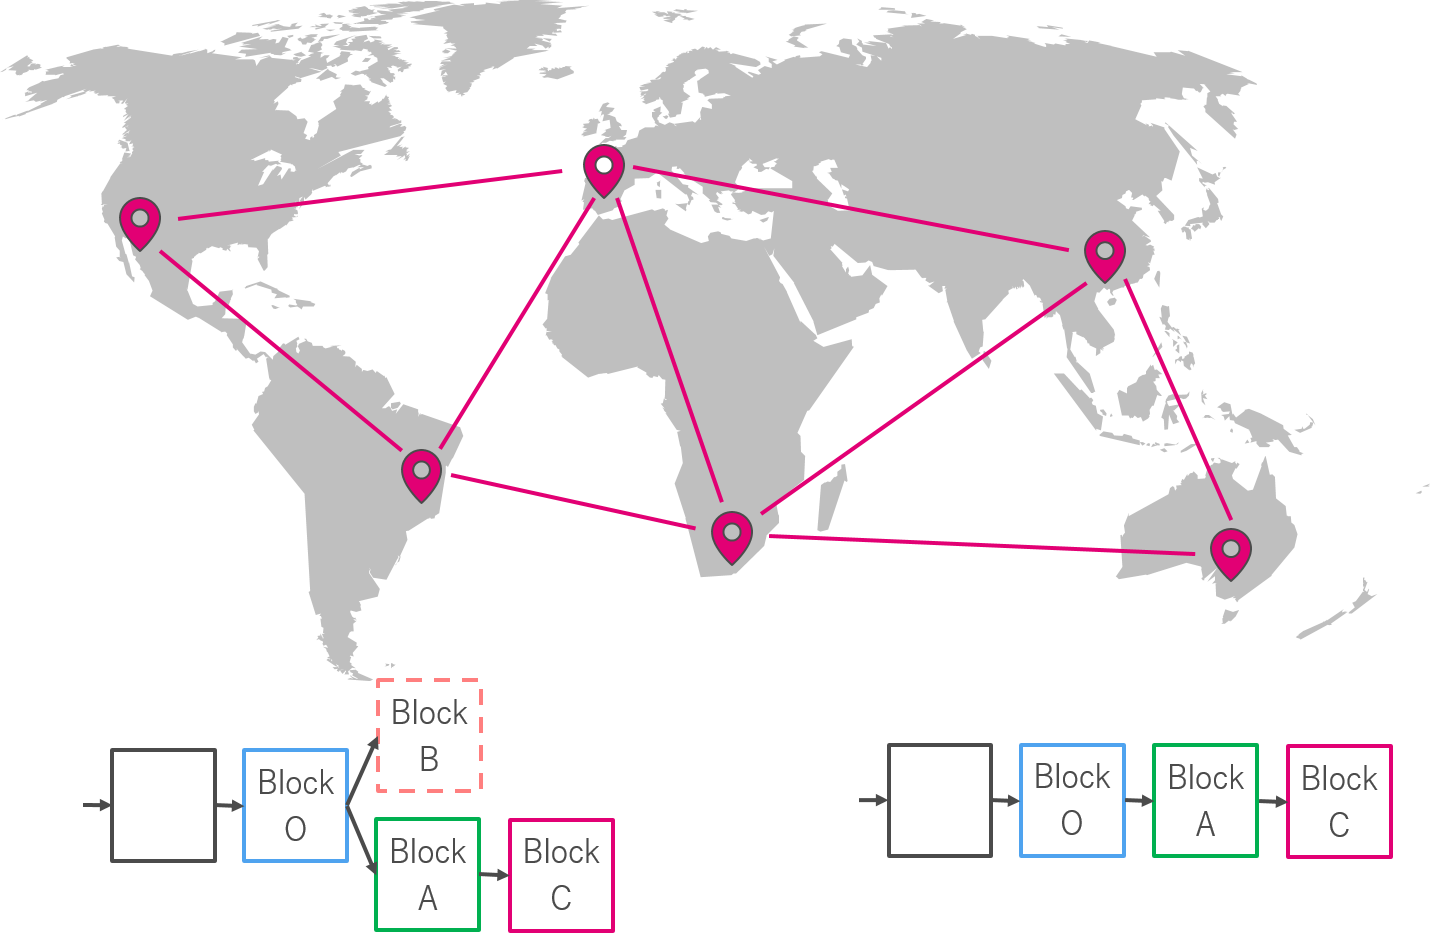
\includegraphics[width=0.95\textwidth,angle=0]{images/fork_4}
 	\caption{Fork-Visualisierung - Block C verbreitet sich im Netzwerk, rote Nodes sehen zwei Blockchains und akzeptieren die längere \cite[S.~200 ff.]{AntonopoulosMasteringbitcoin2015}.}
	\label{fig:fork_4}
\end{figure}

Neben dem \acs{PoW} gibt es noch weitere Konsensmechanismen, wie Proof-of-Stake, Proof-of-Authority oder Practical Byzantine Fault Tolerance \cite{SukhwaniPerformanceModelingPBFT2017a}, \cite{DeAngelisPBFTvsproofofauthority2017} . Diese werden im Kapitel \ref{sec:eval-konsens} genauer beschrieben und analysiert.

\subsubsection{Nichtangreifbarkeit und Unveränderlichkeit}
\label{subsec:immutability}
Viele Faktoren tragen zur Nichtangreifbarkeit und Unveränderlichkeit (im weiteren Verlauf nur noch als Sicherheit bezeichnet) der Blockchain bei. Da alle Nodes die ausgeführten Transaktionen auf Validität prüfen, können diese nicht ohne Berechtigung, im Namen einer anderen Identität oder mit unzureichenden Konditionen ausgeführt werden. Der wichtigste Faktor ist jedoch der genutzte Konsensmechanismus in Verbindung mit den verketteten Blöcken. Durch ihn wird sichergestellt, dass bestehende Daten nicht gelöscht oder manipuliert werden können.

Ein Beispiel dafür kann am \acs{PoW} gezeigt werden. Ein Angreifer probiert eine Transaktion aus einen bestehenden Block zu entfernen. Dazu würde er die Transaktion bei seiner lokalen Blockchain entfernen. Nun ist jedoch der Hash des Blockes sowie der Block selbst nicht valide und würde von keiner Node akzeptiert werden. Der Angreifer muss also erneut einen \acs{PoW} für den manipulierten Block erbringen. Dies wäre für eine Einzelperson jedoch zeitaufwändig. So benötigenm alle Nodes im Bitcoin-Netzwerk im Durchschnitt 10 Minuten, um einen \acs{PoW} zu erbringen \cite[S.~173]{AntonopoulosMasteringbitcoin2015}, bei einer Hash Rate\footnote{Hash Rate: Anzahl der in einer Zeiteinheit berechneten Hashwerte \cite{BitcoinTeamBitcoinGlossar}.} von ca. 13.000.000 TH/s (Terrahashes pro Sekunde) \cite{EtherscanEthereumNetworkHashRate}. Spezielle Hardware für das Mining erreicht hingegen nur eine Hashrate von bis zu 13,5 TH/s \cite{BitcoinminingLearnBitcoinmining}. Wenn der manipulierte Block nun noch Nachfolger hat, muss aufgrund des geänderten Hashes, auch für diese der \acs{PoW} erbracht werden. Hinzu kommt, dass die Blockchain des Angreifers erst dann von allen Nodes akzeptiert wird, wenn sie länger ist, als die aktuell akzeptierte. Er müsste also schneller als das gesamte Bitcoin-Netzwerk Blöcke erschaffen können. Dies ist nur möglich, wenn er 51 \% der Rechenleistung des Netzwerks besitzt. Deshalb wird dieser Angriff auch 51\%-Angriff genannt \cite[S.~83]{SwanBlockchainblueprintnew2015} \cite{EthereumTeamEthereumWhitePaper2017}. 

An dieser Stelle sollte erwähnt werden, dass, auch wenn ein 51\%-Angriff erfolgt, die Angriffsmöglichkeiten beschränkt sind. Der Angreifer kann keine invaliden Transaktionen sowie Blöcke erstellen. Ihm ist es möglich DoS-Angriffe auszuführen, indem er verhindert, dass bestimmte Transaktionen in Blöcken aufgenommen werden. Ebenso kann er die Historie der Daten verändern, indem er eine Transaktion aus einem Block entfernt. Es ist jedoch zu bedenken, dass die Transaktion dabei zurück in den Transaktionspool geht. Er muss also jeden weiteren Block erstellen, um zu verhindern, dass die Transaktion nicht erneut in einen Block aufgenommen wird oder dafür sorgen, dass sie ungültig wird. Im Falle von Kryptowährungen wird ein solcher Angriff Double-Spending-Angriff genannt: Ein Angreifer sendet beispielsweise Bitcoins an einen Händler. Dieser wartet auf die Bestätigung der Transaktion in einen Block sowie auf nachfolgende Blöcke. So stellt er sicher, dass die Transaktion nicht in einem eventuell verworfenen Fork-Branch steht. Erst dann versendet er die Ware. Anschließend ersetzt der Angreifer die Transaktion durch eine Zahlung an sich selbst und erstellt die längere Blockchain. Somit wird die Transaktion an den Händler ungültig, wodurch er letztendlich doch kein Geld erhalten hat \cite{EthereumTeamEthereumWhitePaper2017}. Auch zu bedenken ist, dass ein Nutzer mit 51 \% der Rechenleistung wenig Motivation hat Angriffe auszuführen, da er für jeden erstellten Block Kryptowährung als Belohnung erhält. Ebenfalls würde der Wert dieser sinken, wenn Angriffe auf die Blockchain entdeckt werden. Deshalb besteht für die sogenannten Miner eine Motivation, ehrlich zu arbeiten \cite[S.196 ff.]{AntonopoulosMasteringbitcoin2015}.

Der eben genannte Double-Spending-Angriff kann auf verschiedene Arten durchgeführt werden. So könnte ein Angreifer eine Ware mit Bitcoins bezahlen und diese sofort erhalten. Bevor seine Transaktion jedoch in einen Block besteht, transferiert er die gleichen Bitcoins an sein anderes Konto. Wenn diese beiden Transaktionen letztendlich in einen Block aufgenommen werden sollen, wird eine der Transaktionen ungültig sein, wodurch der Verkäufer eventuell keine Zahlung erhält \cite[S.~211 ff.]{AntonopoulosMasteringbitcoin2015}.

\subsection{Blockchaintypen}
Anhand der zugelassenen Teilnehmer an einer Blockchain ergeben sich 3 Typen. Bisher wurden nur Public Blockchain-Anwendungen, wie Bitcoin und Ethereum, erwähnt. In diesen gibt es keine Teilnehmerbeschränkungen, jeder kann am Netzwerk teilnehmen und die Blockchain öffentlich einsehen. Anders ist dies bei Permissioned (oder auch Consortium \cite{BenHamidaBlockchainEnterpriseOverview2017}) und Private Blockchains. Die beiden Begriffe werden in einigen wissenschaftlichen Arbeiten gleichgesetzt (siehe \cite{Gramolidangerprivateblockchains2016}, \cite{PongnumkulPerformanceAnalysisPrivate2017}, \cite{LiScalablePrivateIndustrial2017}). Hier folgt jedoch eine Unterscheidung. Dabei ist eine Private Blockchain eine Blockchain, welche nur von einem Nutzer verwendet wird. Da eine solche Anwendung keinen Sinn ergibt, da keine Vorteile der Blockchain genutzt werden können, wird darauf nicht genauer eingegangen. Interessanter sind Permissioned Blockchains, an welchen nur zugelassene Nutzer teilnehmen dürfen. Nur diese sind berechtigt, Transaktionen auszuführen und die Daten einzusehen \cite{LiScalablePrivateIndustrial2017}. Dies bietet sich vor allem bei B2B-Anwendungen an, welche von verschiedenen Unternehmen genutzt werden sollen. In solchen kann es beispielsweise aufgrund von sensiblen Daten nötig sein, dass nur bestimmte Parteien Zugriff auf die Blockchain haben. Tabelle \ref{tab:bc-comparison} vergleicht die Blockchaintypen untereinander sowie mit zentralen Datenbanken, da diese am häufigsten für persistente Datenspeicherung genutzt werden. Die dort erwähnten \acs{BFT}-Protokolle werden genauer im Kapitel \ref{sec:eval-konsens} erläutert.

\begin{table}[h]
    \centering
	\begin{tabular}{c c c c}
	\textbf{} & \textbf{Public BC} & \textbf{Permissioned BC}  & \textbf{Zentrale DB} \\ \hline
	Transaktionsdurchsatz & Gering & Hoch & Sehr hoch \\ \hline
    Nicht vertrauenswürdige Nodes & Viele & Wenige & Keine \\ \hline
    Konsensmechanismus & Hauptsächlich \acs{PoW} & \acs{BFT}-Protokolle & Keiner \\ \hline
    Zentral verwaltet & Nein & Teilweise & Ja \\
    \end{tabular}
    \caption{Vergleich der Blockchaintypen mit Datenbanksystemen \cite{WustyouneedBlockchain2017}\cite{ZhengBlockchainChallengesOpportunities2017}.}
	\label{tab:bc-comparison}
\end{table}

\subsection{Exemplarische Anwendungsfälle}
\label{subsec:use-cases}
Die Blockchain wird als revolutionäre Technologie angepriesen (siehe \cite{TapscottBlockchainRevolutionWieTechnologie2016}). Trotzdem ist es wichtig zu wissen, für welche Zwecke sie wirklich geeignet ist. Grundsätzlich ergibt eine Blockchain Sinn, wenn mehrere Parteien, welche sich nicht vertrauen, mit einem System interagieren wollen, welches von keiner dritten, zentralen Instanz verwaltet wird \cite{WustyouneedBlockchain2017}. Um eine bessere Vorstellung von solchen Anwendungen zu erhalten, werden im Folgenden verschiedene exemplarische Anwendungsfälle genannt und beschrieben.

Der erste Anwendungsfall, mit welchem die Blockchain-Technologie auch entstanden ist, sind Kryptowährungen. Mit Ihnen ist es möglich Geld zwischen beliebigen Parteien zu übertragen, ohne dass die Transaktionen von einer eventuell nicht vertrauenswürdigen Bank oder Ähnlichem kontrolliert und verwaltet werden \cite[S.~\Rn{10}]{SwanBlockchainblueprintnew2015}.

Weitere Anwendungsfälle ergeben sich mit der Möglichkeit, Programmlogik auf der Blockchain abzubilden. So können beispielsweise dezentrale Online-Wahlen realisiert werden. Die Stimmen würden in der Blockchain gesammelt werden und können so letztendlich nicht mehr manipuliert werden, beispielsweise von einer korrupten Regierung \cite{CastorEthereumVotingScheme2017}. 

Ein weiterer Anwendungsfall, insbesondere für den B2B-Bereich, wäre Supply Chain Management. Über eine digitale Lieferkette sollen Material- und Informationsflüsse zu Produkten und Dienstleistungen aufgebaut und verwaltet werden \cite{KriegerSupplyChainManagement}. Dies erlaubt Unternehmen das Automatisieren von Prozessen und das verbesserte Reagieren auf Ereignisse (z. B. Lieferverspätungen). Weiterhin ist es dem Unternehmen möglich, dem Kunden exakt aufzuzeigen, wo das Produkt und seine Unterprodukte produziert wurden. In klassischen B2B-Anwendungen müsste jedes Unternehmen, welches ein Teil der Supply Chain ist, die relevanten Daten beispielsweise durch APIs\footnote{API: Schnittstelle für Anwendungsprogrammierung\cite{DigHowAPIsevolve2006}.} bereitstellen. Dies ist mit großen Aufwand verbunden, da diese erstmal entwickelt werden müssen. Weiterhin müssten Plattformen die Daten von unterschiedlichen Schnittstellen abfragen, um diese zusammenzuführen. Aufgrund dieses Aufwandes werden oft Dritte eingestellt, welche sich um den Aufbau und um die Datenintegration der Supply Chain kümmern. Den Aufwand sowie die eventuell nicht vertrauenswürdige dritte Partei könnte durch die Nutzung der Blockchain eliminiert werden. In dieser könnte jedes Unternehmen die relevanten Daten an einer Stelle speichern. Die Supply Chain wäre direkt in der Blockchain vorhanden und kein Unternehmen muss Datenmanipulation oder Ähnliches befürchten \cite{KorpelaDigitalSupplyChain2017}.

Auch dezentrale Märkte sind für B2B-Anwendungen interessant. Der zentrale Marktplattformbetreiber (z. B. Ebay oder Amazon), welcher persönliche Informationen speichert und Gebühren für den Verkauf von Artikeln verlangt, wäre hinfällig. Nutzer könnten Waren untereinander verkaufen, während die Blockchain als Notar für den Warenaustausch dient \cite{BenHamidaBlockchainEnterpriseOverview2017}.

Ein weiteres Beispiel wären Blockchain Sharing-Systeme. So könnte ein dezentrales Fahr-radleihsystem aufgebaut werden. Nutzer würden mit ihrem Smartphone, über ihre in der Blockchain hinterlegte Identität (im Falle von beispielsweise Ethereum die Wallet-Adresse\footnote{Wallet: Speichert beispielsweise bei Ethereum und Bitcoin den Private Key des Nutzers und wird als Adresse für Zahlungen genutzt \cite[S.~61 ff.]{AntonopoulosMasteringbitcoin2015}.}), das Fahrrad entsperren. Dieses erkennt automatisch die gefahrene Distanz sowie die Nutzungsdauer. Über einen Smart Contract würde anschließend die automatische Zahlung erfolgen. Neben der Automatisierung besteht der Vorteil, dass mehrere Unternehmen oder auch Privatpersonen Leihfahrräder anbieten können, ohne dass sie einer zentralen Instanz mit der Verwaltung vertrauen müssen \cite{FutureFluxFestivalBlockchainBikes}, \cite{FischerIoTBlockchain}.

\section{Anforderungen an B2B-Anwendungen}
\label{sec:general-requirements}
Für den zu entwickelnden Prototypen ergeben sich verschiedene Anforderungen, welche zum Teil allgemein für B2B-(Blockchain)-Anwendungen gelten. Es ist wichtig diese zu kennen, um die Blockchain-Technologie in Bezug auf diese zu evaluieren.

\paragraph{Identitätsverwaltung}
Eine B2B-Anwendung besteht zwischen verschiedenen Unternehmen. Die Identitäten dieser müssen bekannt sein, um die Teilnahmeerlaubnis zu erteilen und Berechtigungen zu verwalten. Sie sind ebenfalls von Bedeutung, um ausgeführte Transaktionen den Teilnehmern zuordnen zu können. Die für den Prototypen genutzte Blockchain-Implementierung muss also das Registrieren und Identifizieren von Teilnehmern unterstützen.

\paragraph{Berechtigungsverwaltung}
Die verschiedenen Teilnehmer haben unterschiedliche Rechte was das Lesen, Erstellen und Verändern von Daten betrifft. So ist es beispielsweise wichtig, dass ein Teilnehmer nur seine eigenen, in der Blockchain registrierten, Assets\footnote{Assets: Besitz/Eigentum} verändern kann.

\paragraph{Private Transaktionen}
Bei Blockchains wie Bitcoin und Ethereum sind alle Daten in der Blockchain für alle Teilnehmer einsehbar. Aufgrund von sensiblen Daten kann es allerdings vorkommen, dass nicht alle Transaktionen für alle Teilnehmer sichtbar sein sollen. So sollen beispielsweise Preisabsprachen nur von den relevanten Unternehmen eingesehen werden können.

\paragraph{Skalierbarkeit und Performance}
In Bitcoin ist lediglich ein Transaktionsdurchsatz von 7 \acl{TPS} (\acs{TPS}) möglich \cite{ZhengBlockchainChallengesOpportunities2017}. Hinzu kommt, dass es ca. zwischen 30 Minuten und 16 Stunden dauern kann, bis eine Transaktion bestätigt ist \cite{BuchkoHowLongBitcoin2017}. Darauf wird auch genauer im Kapitel \ref{sec:scalability-eval} eingegangen. In B2B-Anwendungen kann die Performance und Skalierbarkeit von großer Bedeutung sein. Je nach Art der Anwendung und Anzahl der Teilnehmer muss ein höherer Transaktionsdurchsatz als bei Bitcoin erzielt werden. Die Skalierbarkeit ist vor allem beim Einsatz von IoT-Geräten von Bedeutung, welche untereinander kommunizieren und Transaktionen ausführen. Gartner behauptet, dass es bis 2020 ca. 7,5 Billionen vernetzte Geräte im Business-Sektor geben wird \cite{RobGartnerSaysBillion2017}. Damit wäre ein Transaktionsdurchsatz von 7 TPS nicht praktikabel.

\paragraph{Sicherheit}
Die Sicherheit wird durch den genutzten Konsensmechanismus realisiert. Der am häufigsten genutzte \acs{PoW} ist in einem Netzwerk mit wenig Teilnehmern allerdings unsicher, da es einfach ist 51 \% der Rechenleistung zu erreichen. Weiterhin führt er zu einen hohen Stromverbrauch (im Bitcoin-Netzwerk der Verbrauch von ca. 3.500.000 US-Haushalten \cite{DigiconomistBitcoinEnergyConsumption}), welcher nicht erwünscht ist. Ebenfalls beeinflusst der \acs{PoW} die Performance (siehe Kapitel \ref{cha:b2b-eval}).



	
\chapter{Aktueller Stand der Technik}
\label{cha:stand-technik}

Die Blockchain-Technologie ist im Jahr 2008 entstanden. Jedoch befindet sie sich erst seit ca. 2016 in einem Hype, wie die Gartner Hype Cycle von 2016 und 2017 \cite{PanettaTopTrendsGartner2017}\cite{AmyGartner2016Hype2016} sowie die Google Trends zum Suchinteresse \cite{GoogleBlockchainGoogleTrends18} zeigen. Aufgrund des Hypes entstehen viele Ideen zu der möglichen Anwendung der Blockchain, darunter auch viele unnütze \cite{WustyouneedBlockchain2017}. Im Gartner Hype Cycle ist dies die ``Peak of Inflated Expectations''. Es bestehen unrealistische Erwartungen an die Technologie, und die Anwendungszwecke sind noch nicht klar. 

Es finden sich wenig Blockchain-Anwendungen, welche bereits in Produktionsumgebungen eingesetzt werden. Dies liegt u.a. auch daran, dass es sich um eine relativ junge Technologie handelt. Viele Blockchain-Implementationen werden nur für Kryptowährungen eingesetzt. Dazu gehören z.B. Bitcoin, Monero, Dashcoin oder Litecoin \cite{BlockchainHubBlockchainsDistributedLedger}. Erst mit Ethereum wird das Konzept von Smart Contracts erfolgreich implementiert, womit es möglich ist eigene Programmlogik in der Ethereum-Blockchain abzubilden und so dezentrale Anwendungen zu entwickeln. So nutzt beispielsweise AXA diese für Flugversicherungen. Kommt es zu einer bestimmten Verspätung eines Fluges löst ein Smart Contract automatisch die Auszahlung an den Kunden aus \cite{BoerAXAnutztEthereumBlockchain2017}. Während es viele Ideen für dezentralisierte Anwendungen gibt, handelt es sich bei vielen nur um Prototypen.

Ein weiteres Problem an jungen Technologien ist, dass die Limitationen noch nicht komplett evaluiert und gelöst sind. Dies führt dazu, dass die Blockchain für bestimmte Anwendungen (noch) nicht geeignet ist. Die Probleme werden in diversen wissenschaftlichen Arbeiten analysiert und es werden Lösungen für diese vorgeschlagen (Siehe \cite{ZhengBlockchainChallengesOpportunities2017}, \cite{SwanBlockchainblueprintnew2015} und \cite{SchererPerformanceScalabilityBlockchain2017}). Tweilweise handelt es sich jedoch nur um Vorschläge, welche sich noch nicht im Einsatz befinden. Kapitel \ref{cha:b2b-eval} beschäftigt sich genauer mit den Problemen, welche die Blockchain mit sich bringt.

Für Permissioned Blockchains haben sich verschiedene Plattformen herausgebildet. So gibt es Multichain, Quorum, Hyperledger Fabric oder Hyperledger Burrow \cite{BenHamidaBlockchainEnterpriseOverview2017}. Diese sollen die Probleme der öffentlichen Blockchains lösen. Aber auch hier gilt es die Implementationen genauer zu analysieren, um eine Aussage über ihren Nutzen zu treffen. So setzen sich Arbeiten von \cite{BenHamidaBlockchainEnterpriseOverview2017}\cite{LiScalablePrivateIndustrial2017}, \cite{PongnumkulPerformanceAnalysisPrivate2017} und \cite{VukolicRethinkingPermissionedBlockchains2017} u.a. mit der Skalierbarkeit und Performance der Permissioned Blockchains auseinander.

Dezentrale Märkte sind eine der am meisten mit Blockchain in Verbindung erwähnten Use-Cases, wie man an Quellen wie \cite{BenHamidaBlockchainEnterpriseOverview2017} und \cite{RavalDecentralizedApplicationsHarnessing2016} sehen kann.
Neben Konzepten für diese (Siehe \cite{KaiserDecentralizedPrivateMarketplace}), gibt es auch Live-Systeme, wie Syscoin \cite{SidhuSyscoinPeertoPeerElectronic2017}.

Dezentrale Wartungsmärkte hingegen werden nur in Verbindung mit der Supply Chain erwähnt, wie zum Beispiel in \cite{SoldatosWhatDoesBlockchain2017} oder \cite{GotzeLufthansaIndustrySolutions}. Implementationen oder Konzeptentwürfe konnten nicht gefunden werden.





\chapter{Evaluierung Permissioned Blockchains für B2B}
\label{cha:b2b-eval}

Die Blockchain-Technologie bringt diverse Probleme mit sich, welche je nach Anwendungszweck und Blockchaintyp verschieden große Auswirkungen haben. Für den B2B-Bereich gilt es vor allem die Skalierbarkeit sowie die Konsensmechanismen zu analysieren.

\section{Skalierbarkeit}
\label{sec:scalability-eval}
Das CAP-Theorem besagt, dass es in einem verteilten System nur möglich ist, zwei von den drei folgenden Eigenschaften zu erfüllen: Konsistenz, Verfügbarkeit und Ausfalltoleranz. Bezogen auf die Blockchain wären dies: Dezentralisierung, Skalierbarkeit und Nichtangreifbarkeit \cite{SchererPerformanceScalabilityBlockchain2017}. Im Zuge der Skalierbarkeit wird vor allem auf den Performance (Transaktionsdurchsatz), sowie die Anzahl von Nutzern  eingegangen. Dazu erfolgt zunächst eine Analyse an aktuellen Public Blockchains, und letztendlich an Permissioned Blockchains. Als Referenzwerte werden die Transaktionsdurchsätze von Paypal und Visa genutzt. Die Ergebnisse werden ebenfalls auf das CAP-Theorem angewandt.  

\subsection{Public Blockchains}
%TODO: Eventuell entfernen
\begin{figure}[!htbp]
  \centering
    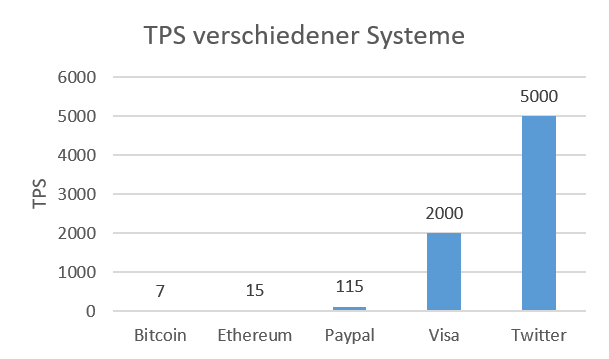
\includegraphics[width=0.85\textwidth,angle=0]{images/tps-comparison}
     \caption{Möglicher Transaktionsdurchsatz bei Bitcoin, Ethereum, Paypal und Visa \cite{BitcoinTeamScalabilityBitcoinWiki}.}
    \label{fig:tps-comparison}
\end{figure}

\subsubsection{Bitcoin}
Das Bitcoin-Netzwerk erreicht aktuell einen maximalen Transaktionsdurchsatz von 7 Transaktionen (unterschiedlich je nach Größe der Transaktionen, variiert zwischen ungefähr 0,5kb und 1,2kb \cite{Bitcoin.comTeamBitcoinTransactionSize}) pro Sekunde (TPS), bei einer Blockgröße von 1MB. Hingegen erreichen Paypal und Visa zu Spitzenzeiten 115 TPS und 2000 TPS (siehe auch Abb. \ref{fig:tps-comparison}) \cite{BitcoinTeamScalabilityBitcoinWiki}. Hinzu kommt, dass ungefähr 170000 unbestätigte Transaktionen\footnote{Unbestätigte Transaktion: Eine Transaktion, welche noch nicht in einen Block vorkommt \cite{AntonopoulosMasteringbitcoin2015}.} bestehen \cite{BlockchainUnternehmenUnbestatigteTransaktionenBitcoin}. Berechnungen von Scherer zeigen, dass bei 11,8 Millionen Nutzern im Bitcoin-Netzwerk, sowie einem Transaktionsdurchsatz von 4 TPS, jeder Nutzer nur nur ca. 10 Transaktionen im Jahr senden kann \cite{SchererPerformanceScalabilityBlockchain2017}.

Der Transaktionsdurchsatz ist durch verschiedene Faktoren limitiert. Hauptsächlich durch die limitierte Blockgröße von 1MB, und dem PoW: Nur eine bestimmte Anzahl an Transaktionen passt in einen Block, und nur alle 10 Minuten wird einer erstellt. Es gäbe also die Möglichkeit, die Blockgröße zu vergrößern, oder die Zeit für den PoW zu verringern, indem die Schwierigkeit angepasst wird. Es gibt jedoch diverse Nachteile, welche dadurch entstehen würden. Bei einer größeren Blockgröße würde es länger dauern, bis ein Block beim Propagieren durch das Netzwerk alle Nodes erreicht. Dies würde zu öfter vorkommenden und längeren Forks führen und somit die Sicherheit des Netzwerks beeinträchtigen. Den gleichen Effekt hätte eine kürzere PoW Zeit, da die Wahrscheinlichkeit höher ist, dass zwei Nodes zur ungefähr gleichen Zeit einen Block erstellen \cite{SchererPerformanceScalabilityBlockchain2017} \cite{EthereumTeamEthereumWhitePaper2017} \cite{SompolinskyAcceleratingBitcoinTransaction2013}. 

Entsteht ein Fork, probieren Nodes die längere und somit gültige Blockchain zu erschaffen. Gelingt dies, wird die kürzere Blockchain mit den nun sogenannten Stale Blocks verworfen. Die gesamte Rechenleistung, welche in die Stale Blocks und seine Nachfolger geflossen ist, trägt nicht zur Sicherheit des Netzwerks bei. Dies lässt sich auch anhand der Abbildung \ref{fig:forking-risks} erläutern. Innerhalb der Blockchain bestehen durch mehrere Forks 5 Branches. Das bedeutet, dass die Rechenleistung des Netzwerks auf diese aufgespalten ist. Es wird davon ausgegangen, dass 20\% der Rechenleistung in den obersten Branch geflossen ist, welcher der längste ist. Die restlichen 4 Branches erhalten je 10\% der Rechenleistung. Wenn es nun einen Angreifer mit 40\% der Rechenleistung probiert eine eigene Blockchain zu erstellen, gelingt ihm dies, da er schneller die längere Blockchain erstellen kann \cite{SompolinskyAcceleratingBitcoinTransaction2013}. Zusammenfassend lässt sich sagen, dass ein Angreifer nicht 51\% der Rechenleistung für einen Fork benötigt, wenn das Netzwerk diese bei Forks verschwendet \cite{Buterin12secondBlockTime2014}. 

Ein weiteres Problem der Forks ist, dass Miner keine Belohnung für die Arbeit an verworfenen Blöcken erhalten. Dadurch kann es zur Zentralisierung durch wachsende Mining Pools kommen. Dies wird an folgenden Beispiel ersichtlich: Ein Mining Pool A besitzt 30\% der Rechenleistung, ein Mining Pool B 10\%. In dem genannten Beispiel würde Mining Pool A in 70\% aller Fälle einen Stale Block erzeugen, und B in 90\% aller Fälle. Kein Miner würde dem Mining Pool B beitreten, da die Wahrscheinlichkeit geringer ist, dass B gültige Blöcke erschafft. A hingegen würde immer mehr Miner, und somit mehr Rechenleistung erhalten \cite{EthereumTeamEthereumWhitePaper2017}.

An dieser Stelle sollte auch darauf hingewiesen werden, dass schnellere Blockerstellungszeiten nicht zwingend zu schnelleren Transaktionsbetätigungen führen. Transaktionen werden zwar schneller in Blöcken aufgenommen, aber es muss auf mehr Nachfolger gewartet werden, um sicher zu gehen, dass die Transaktion nicht in einem Fork vorkommt \cite{SchererPerformanceScalabilityBlockchain2017}.

\subsection{Ethereum}

\paragraph{Bessere Skalierbarkeit durch GHOST}
Das Ethereum Netzwerk nutzt das sogenannte GHOST-Protokoll, und erreicht damit eine Transaktionsdurchsatz von 15 TPS, bei einer durchschnittlichen Zeit von 15 Sekunden um den PoW zu erbringen. Dieses löst Probleme des Forkings und der Benachteiligung von Minern. Ersteres wird dadurch gelöst, dass Stale Blocks in die Berechnung der gültigen Blockchain einfließen. Anders als bei Bitcoin, wo lediglich die Parents und deren Nachfolger eine Rolle spielen. Die Stale Blocks werden in Ethereum ``Uncles'' genannt. Kurz gesagt, ist ein Uncle ein alternativer gefundener Block welcher auf der gleichen Höhe wie der Parent bestehen würde \cite{EthereumTeamEthereumWhitePaper2017}.

Die Bestimmung der gültigen Blockchain wird an der Abbildung \ref{fig:forking-risks} ersichtlich. In Ethereum ist die Blockchain die gültige, für welche die meiste Arbeit aufgebracht wurde, unter Einbezug der Uncles. Das führt dazu, dass der Branch mit den meisten Uncles bestehen bleibt. Das bedeutet letztendlich, dass die gesamte Rechenleistung das Netzwerk absichert, auch wenn diese sich auf die Branches aufteilt. Ein Angreifer braucht somit weiterhin 51\% der Rechenleistung um einen Angriff auszuführen \cite{SompolinskyAcceleratingBitcoinTransaction2013}.

\begin{figure}[!htbp]
  \centering
    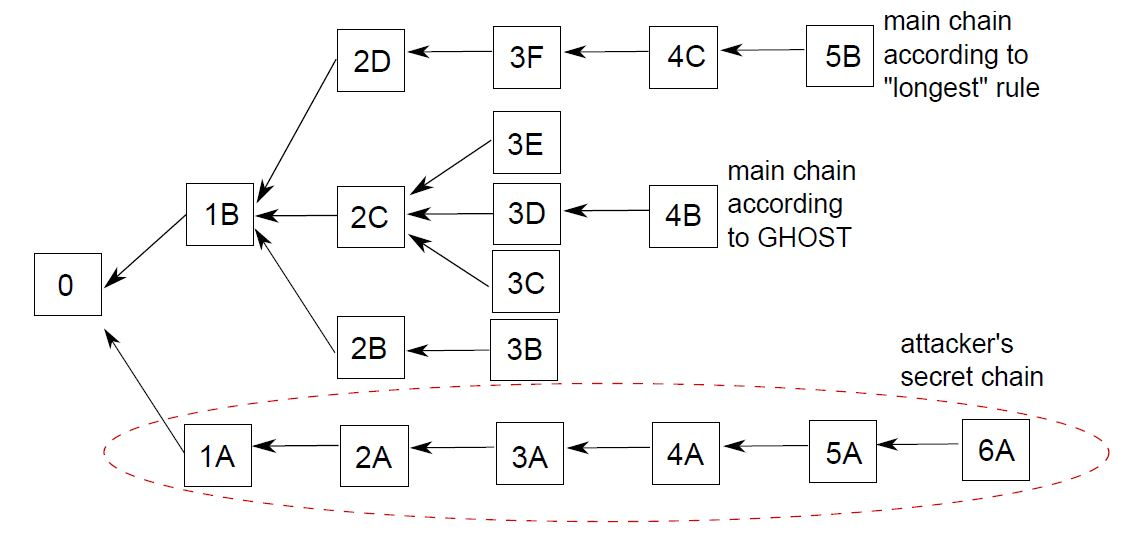
\includegraphics[width=0.8\textwidth,angle=0]{images/forking-risks}
     \caption{Auswahl der gültigen Blockchain. Bei Bitcoin die längere. Bei Ethereum die mit der meisten erbrachten Arbeit, unter Einberechnung der Uncle-Blocks \cite{SompolinskyAcceleratingBitcoinTransaction2013}.}
    \label{fig:forking-risks}
\end{figure} 

Damit ist allerdings noch nicht das Problem der Zentralisierung durch Mining Pools gelöst. Es besteht weiterhin keine Motivation für Miner, Uncles zu minen. Deswegen ist das GHOST-Protokoll in Ethereum so erweitert, dass Miner Ether\footnote{Kryptowährung von Ethereum \cite{EthereumTeamEthereumWhitePaper2017}.} als Belohnung für das Erstellen von Uncles erhalten (allerdings weniger als bei vollwertigen Blöcken). Somit besteht ebenfalls die Motivation, kleineren Mining Pools beizutreten \cite{EthereumTeamEthereumWhitePaper2017}. An dieser Stelle sollte auch erwähnt werden, dass Miner entscheiden können, an welchen Branch sie arbeiten \cite{ZhengBlockchainChallengesOpportunities2017}.

Während Ethereum die Probleme löst, welche durch Forks entstehen, ist der Transaktionsdurchsatz trotzdem limitiert. Die Blockgröße muss klein genug bleiben, damit das Propagieren im Netzwerk effizient bleibt \cite{SchererPerformanceScalabilityBlockchain2017}. Ansonsten würden Miner unter Umständen so benachteiligt werden, dass sie nur sehr selten bis garnicht den aktuellen Block der gültigen Blockchain erhalten würden. Dies wiederum würde dazu führen, dass sie nur Uncles minen können, und so nie die volle Belohnung erhalten können. Hinzu kommt, das Uncles nur gültig sind, wenn sie maximal eine bestimmte Anzahl an Generationen vom aktuellen Block in der gültigen Chain entfernt sind. Ansonsten hätten die Miner auch weniger Motivation ehrlich zu bleiben, da sie ohne Nachteile an der Chain eines Angreifers arbeiten könnten \cite{EthereumTeamEthereumWhitePaper2017}.

\paragraph{Schlechtere Skalierbarkeit durch Smart Contracts}
Ethereum löst die Probleme von häufig auftretenden Forks und erlaubt so einen höheren Transaktionsdurchsatz sowie schnellere Transaktionsbestätigungszeiten. Weitere Probleme entstehen jedoch, wenn eine Blockchain nicht nur Geldtransfertransaktionen verarbeitet. Ethereum erlaubt das speichern und ausführen von eigenem Code durch Smart Contracts. Dadurch steigt die Komplexität der auszuführenden Transaktionen. Dadurch nimmt die Performance ab, da die entstehenden größeren Blöcke eine längere Propagationszeit verursachen. Ebenfalls verschlechtert sich die Performance des Netzwerks, da die Daten schwieriger zu verarbeiten sind. So muss jede Node alle Transaktionen verifizieren, Smart Contract-Code ausführen, und die Ergebnisse speichern. \cite{SchererPerformanceScalabilityBlockchain2017}. 

In Ethereum werden Transaktionen sequentiell bei allen Nodes ausgeführt. Dazu gehört das ausführen von Smart Contract-Code sowie das verifizieren der Ergebnisse. Nur so können in Konflikt stehende Transaktionen, wie zum Beispiel beim Double-Spend) erkannt werden. Eine Parallelausführung ist nicht möglich. Dies verschlechtert letztendlich die Performance des Netzwerks, da es länger dauert Transaktionen auszuführen \cite{SchererPerformanceScalabilityBlockchain2017}. Dies wird auch durch ein Beispiel klar. Ein Angreifer kann DoS-Attacken ausführen, indem er komplex auszuführende Smart Contracts schreiben. Die Ausführung von diesem bei jeder Node führt dazu, dass keine anderen Operationen ausgeführt werden können. Ethereum löst dieses Problem, indem der Transaktionssender für jeden Berechnungschritt eine Gebühr zahlen muss. Dies funktioniert jedoch nur, wenn in der Blockchain-Anwendung eine Kryptowährung genutzt wird \cite{VukolicRethinkingPermissionedBlockchains2017}. 

Ebenfalls behauptet Vukolic, dass der Code der Smart Contracts nicht bei allen Nodes ausgeführt werden muss. Um Konsens zu erreichen genügt es, dass alle Nodes den gleichen Stand der Daten erhalten. Deshalb könnte die Codeausführung von nur von bestimmten Nodes ausgeführt werden. Das Problem dabei ist, dass man eine genügend große Anzahl an vertrauenswürdige Teilnehmer festlegen muss \cite{VukolicRethinkingPermissionedBlockchains2017}. Damit geht allerdings auch das vertrauenslose Modell der Blockchain verloren.

Letztendlich lässt sich sagen, dass Public Blockchains nicht skalieren . Um dies zu lösen, müssen  schnellere Blockpropagrationszeiten, geringere Transaktionsgrößen und/oder bessere Transaktionsverarbeitung realisiert werden \cite{SchererPerformanceScalabilityBlockchain2017}. Weitere Schwierigkeiten bestehen sobald nicht nur Geldtransferaktionen verarbeitet werden müssen. Betrachtet man das CAP-Theorem wird ersichtlich, dass nur die Eigenschaften Dezentralisierung und Sicherheit gegeben sind. Es ist jedoch zu bedenken, dass viele Probleme der Skalierbarkeit aufgrund der genutzten Konsensmechanik bestehen. Auch wenn es teilweise Lösungsvorschläge für diese gibt, genügen sie bisher nicht um Skalierbarkeit herzustellen. Deshalb gilt es, die Limitationen von Permissioned Blockchains sowie alternative Konsensmechaniken für diese zu analysieren.

%MinPermissioned: Introduces a concept for better throughput, but it is not tested (??)
%S.1-6 LiScalable: Introducing a concept with sattelite chains

\subsection{Permissioned Blockchains}
Permissioned Blockchains werden eingesetzt, wenn nur bestimmte Teilnehmer an der Blockchain teilnehmen sollen. So gibt es z.B. auch eine verwaltende Instanz, welche u.a. die ersten berechtigten Teilnehmer bestimmt und die Netzwerkkonfiguration vornimmt. Dadurch entsteht eine stärkere Zentralisierung als bei Public Blockchains. Bezieht man sich auf das CAP-Theorem, müssten sich dadurch die Sicherheit und/oder Skalierbarkeit verbessern. Dies führt allerdings auch dazu, dass ein größeres Maß an Vertrauen zwischen den Teilnehmern gegeben sein muss. Dies wird dadurch sichergestellt, dass jeder Teilnehmer die Rechte zur Teilnahme am Netzwerk erhalten hat und die Identitäten dieser bekannt sind. Durch letzteres ist nachverfolgbar, welche Teilnehmer welche Transaktionen ausführen \cite{SchererPerformanceScalabilityBlockchain2017}.

Scherer behauptet, dass das größere Vertrauen es erlaubt den Nodes verschiedene Aufgaben zuzuteilen. Dies beschreibt er am Beispiel von Hyperledger Fabric, einer Permissioned-Blockchain. In dieser gibt es Peer und Ordering Nodes. Erstere simulieren das ausführen von der Transaktionen und der damit verbundenen Datenänderungen. Letztere bestimmen die Reihenfolge der auszuführenden Transaktionen in den Blöcken. Peer Nodes führen die bereits simulierten Transaktionen nacheinander aus und erkennen Konflikte in den Transaktionen (genauer im Kapitel \ref{sec:hyperledger-fabric-composer} erklärt). Die Ordering Nodes sind also letztendlich für den Konsens verantwortlich. In Gegensatz zu Ethereum können Peer Nodes so parallel Transaktionen verarbeiten. Sie müssen sich nicht um eventuelle Konflikte oder die Reihenfolge der Transaktionen kümmern. Letztendlich würde die Skalierbarkeit, von der Hardware der Peers und der Anzahl dieser abhängen.

%TODO: Warum müssen die Endorser kommunizieren ?
Scherer führt ebenfalls Tests durch um die Performance von Hyperledger Fabric zu analysieren. Dazu nutzt er eine frühe und unstabile Version 1.0. Das Netzwerk besteht aus einer Ordering und einer Peer Node. Es wird kein Konsensmechanismus genutzt. Die Anwendung selber unterstützt die Zahlung mittels digitaler Assets (z.B. Tokens bzw. Coins) zwischen zwei Accounts. Dabei erreicht er einen maximalen Transaktionsdurchsatz von 350 TPS. Dabei ist allerdings zu bedenken, dass der Test auf einer Maschine mit limitierten Ressourcen ausgeführt wird. Um einen maximalen Transaktionsdurchsatz zu erreichen, müssten mehrere leistungsstarke Computer für den Test eingesetzt werden. Scherer stellt ebenfalls fest, dass der Transaktionsdurchsatz abnimmt, desto mehr Peers es gibt, welche Transaktionen bestätigen. Dies liegt daran, dass diese sogenannten Endorser untereinander kommunizieren müssen. Pro Node müssten O(n$^2$) Nachrichten gesendet werden, wobei n die Anzahl an Nodes ist. Die Anzahl an effizient nutzbaren Endorsern ist also beschränkt. So führt der Test mit einen Endorser zu einen Transaktionsdurchsatz von ca. 70 TPS, während mit 14 Endorsern nur noch ca. 15 TPS erreicht werden. Somit wäre die Anzahl an effizient nutzbaren Endorsern begrenzt. Scherer behauptet jedoch, dass Fabric mit rechenstarken Maschinen in der Theorie tausende TPS unterstützt \cite{SchererPerformanceScalabilityBlockchain2017}.

Ein Paper von Pongnumkul u. a. vergleicht die Leistung von Hyperledger Fabric mit Ethereum. Er nutzt dazu die stabile Version 0.6. Er führt die Test ebenfalls mit nur einer Peer Node durch. Zur Ordering Node macht er keine Angabe. Die Anwendung ist die gleiche wie bei Scherer und es wird ebenfalls kein Konsensmechanismus genutzt. Pongnumkul stellt fest, dass die Performance von Fabric in allen Kriterien besser ist als bei Ethereum. So betrug die Zeit, bis eine Beispieltransaktion verarbeitet wurde bei Ethereum 41 Sekunden und bei Ethereum 478 Sekunden. Tests zum maximalen Transaktionsdurchsatz haben ergeben, dass Ethereum 40 TPS und Hyperledger Fabric 300 TPS erreicht hat. Die dazugehörige Abbildung \ref{fig:tps-ethereum-vs-hyperledger} zeigt auch, dass die Unterschiede zwischen Ethereum und Fabric signifikanter sind, desto mehr Transaktionen verarbeitet werden müssen \cite{PongnumkulPerformanceAnalysisPrivate2017}.

\begin{figure}[!htbp]
  \centering
    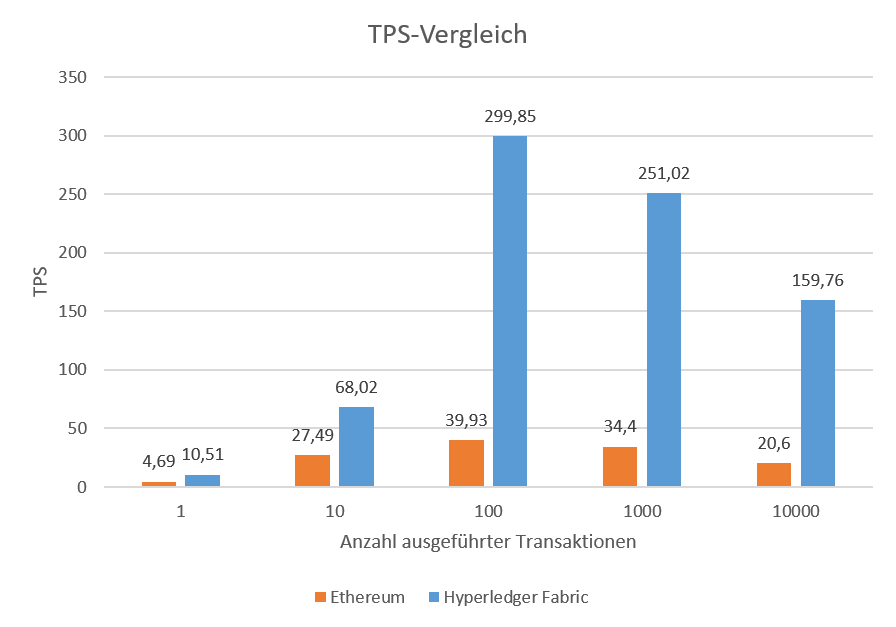
\includegraphics[width=0.8\textwidth,angle=0]{images/tps-ethvshyp}
     \caption{Vergleich des Transaktionsdurchsatzes von Ethereum und Hyperledger Fabric \cite{PongnumkulPerformanceAnalysisPrivate2017}.}
    \label{fig:tps-ethereum-vs-hyperledger}
\end{figure} 

Bei beiden Tests ist zu bedenken, dass sie mit nicht aktuellen Versionen von Hyperledger Fabric ausgeführt wurden. Mittlerweile gibt es eine stabile Version 1.0, sowie eine Preview von Version 1.1.0 \cite{HyperledgerFabricTeamHyperledgerFabricReleases2018}. Es ist also möglich das die Performance sich mittlerweile verbessert hat.

Letztendlich lässt sich sagen, dass Permissioned Blockchains, was die Verarbeitung von Transaktionen betrifft, eine bessere Performance erzielen. Damit bestätigt sich auch das CAP-Theorem bezüglich der Skalierbarkeit. Die Performance wurde allerdings noch nicht unter der Nutzung verschiedener Konsensmechanismen betrachtet. Weiterhin muss das CAP-Theorem noch auf die Sicherheit untersucht werden. Deshalb erfolgt im nächsten Kapitel die Analyse der Skalierbarkeit und Sicherheit von Konsensmechanismen.

%TODO: Add Raft/Kafka ?
\section{Konsensmechanismen}
\label{sec:eval-konsens}
Das Erreichen von Konsens in einer Blockchain, ist eine Abwandlung des Byzantine Generals Problem. In diesem gibt es Generäle, welche Armeen kommandieren welche eine Stadt umzingeln. Ein Angriff auf diese ist nur erfolgreich, wenn alle Armeen gleichzeitig angreifen. Die Generäle müssen untereinander kommunizieren und Konsens darüber herstellen, ob ein Angriff erfolgen soll. Allerdings gibt es Verräter unter diesen. Es handelt sich also um ein vertrauensloses Umfeld. Genau so kann es in einer Blockchain zu den sogenannten Byzantine Faults kommen, wenn nicht vertrauenswürdige Nodes Daten manipulieren können. Deshalb müssen verteilte Systeme Byzantine Fault Tolerance (BFT) herstellen, um eine gewisse Anzahl an nicht vertrauenswürdigen Teilnehmern zu tolerieren. Dies geschieht in Blockchains über die Konsensmechanismen \cite{ZhengBlockchainChallengesOpportunities2017}.

Eine Blockchain, welche den PoW als Konsensmechanismus nutzt, ist nicht skalierbar. Ebenfalls würde er in Netzwerken mit relativ wenig Teilnehmern die Sicherheit beeinträchtigen, da ein Teilnehmer einfacher 51\% der Rechenleistung erreichen kann. Für Permissioned Blockchains muss also ein Konsensmechanismus gefunden werden, welche Skalierbarkeit und Sicherheit herstellt. Aufgrund des höheren Vertrauens in Permissioned Blockchains, behauptet Scherer, dass ein Konsensmechanismus genutzt werden kann, welcher Vertrauen in geringerem Maße als der PoW garantiert. Somit könnten Skalierbarkeit und Sicherheit hergestellt werden \cite{SchererPerformanceScalabilityBlockchain2017}. Im folgenden werden verschiedene Konsensmechanismen verschiedener Blockchain-Technologien miteinander verglichen. Dabei ist zu bedenken, dass nur auf die Konsensmechanismen, welche Sicherheit und Skalierbarkeit in Permissioned Blockchains sicherstellen können, im Detail eingegangen wird.

\subsection{Proof of Stake}
Beim PoS hängt die Wahrscheinlichkeit, einen Block zu minen, von der Menge des Eigentums (z.B. Kryptowährung) eines Nutzers ab. Desto mehr Bitcoins man beispielsweise hat, desto höher ist die Wahrscheinlichkeit für das Mining ausgewählt zu werden. Ähnlich wie beim PoW könnte ein Teilnehmer mit 51\% aller Bitcoins das Netzwerk angreifen, da er die längere Blockchain erstellen kann. Aber selbst wenn es ein Teilnehmer schafft, 51\% der Bitcoins zu besitzen, hätte er keine Motivation dazu. Denn letztendlich würde ein Angriff den Kurs von Bitcoin senken, und somit würde der Miner sich selber schaden \cite{ZhengBlockchainChallengesOpportunities2017}. Da der PoS hauptsächlich nur bei Kryptowährungen genutzt werden kann, ist er für Permissioned Blockchains uninteressant.

\subsection{Proof of Elapsed Time}
Der PoET wird in Intels Blockchain-Technologie Hyperledger Sawtooth genutzt. Die grundlegende Idee ist, dass eine Node eine zufällige Zeit generiert, welche Sie warten muss um einen Block zu erstellen. Um sicherzustellen, dass die generierte Zeit nicht verfälscht wurde, wird Trusted Computing \footnote{Trusted Computing: Hardware, welche sicher stellt, dass ein Computer sich wie erwartet verhält \cite{MitchellTrustedComputing2005}} genutzt. So stellen Intels Software Guard Extensions (SGX) sicher, dass Code nicht modifiziert werden kann. Eine Node muss also über solchen unmodifizierbaren Code eine Zeit generieren. Weiterhin erfolgen statistische Tests, um zu verhindern dass eine Node Blöcke zu schnell und somit zu oft erstellt. Letztendlich ist die Blockerstellung damit fair verteilt, und kein Teilnehmer kann die Blockchain kontrollieren. Im Prinzip funktioniert der Mechanismus wie der PoW. Dort wird eine Wartezeit durch das Finden eines Hashes sichergestellt, während dies beim PoET durch die Hardware sichergestellt wird. Dadurch, dass es keine rechenintensiven Aufgaben gibt, ist die Skalierbarkeit sicher gestellt. Es ist jedoch zu bedenken, dass es bisher wenige Analysen zu der Sicherheit des PoET gibt. Ein Paper von Chen u. a. stellt fest, dass der Konsensmechanismus unter bestimmten Umständen unsicher ist, schlägt aber auch Lösungen dafür vor. Ebenfalls kommt hinzu, dass man der Hardware von Intel für das Trusted Computing vertrauen muss. \cite{ChenSecurityAnalysisProofofElapsedTime2017}.

\subsection{Diversity Mining Consensus}
Der Diversity Mining Consensus ist ähnlich dem PoW. In diesem ist der Block einer Node nur valide, wenn sie eine bestimmte Anzahl an vorherigen Blöcken nicht erstellt hat. Dies führt letztendlich dazu, dass eine Wartezeit für jede Node nicht durch das Finden eines Hashes (siehe PoW) oder durch eine generierte Zeit (siehe PoET) realisiert wird. Für den Mechanismus müssen alle Teilnehmer am Netzwerk bekannt sein. Auch hier kann es zu Forks kommen, wenn zwei Nodes zur ungefähr gleichen Zeit einen Block erstellen. Ebenfalls wird die entstehende längere Blockchain akzeptiert. Durch die Wartezeit wird sichergestellt, dass der Branch mit den meisten Minern die längere Blockchain erstellt. Die Gefahr bei diesen Konsensmechanismus ist, dass bösartige Miner sich zusammen tun können. Unter den richtigen Umständen erstellt der Zusammenschluss die meisten Blöcke, und kann somit auch bei Forks eine längere Blockchain erstellen, um so Double-Spend-Angriffe auszuführen. Die Skalierbarkeit ist aufgrund des fehlenden Rechenaufwands gegeben. \cite{GreenspanMultiChainPrivateBlockchain2015}\cite{CachinBlockchainConsensusProtocols2017}.

\subsection{QuorumChain}
Quorum ist ein Fork von Ethereum für Permissioned Blockchains. Dieser nutzt den Konsensmechanismus QuorumChain. Es gibt Voter und Block-Maker Nodes. Die Block-Maker schlagen Blöcke zum erstellen vor, und die Voter stimmen für diese ab. Um Forks zu verhindern, warten die Block-Maker eine zufällige Zeit und erstellen den Block. Die Voter validieren diesen und stimmen für ihn ab, indem Sie u.a. die Transaktionen ausführen und überprüfen ob der vorherige Block genug Stimmen erhalten hat. Die Nodes hängen letztendlich den Block an ihre lokale Chain an, welcher einen bestimmten Schwellwert an Stimmen überschritten hat, oder im Falle eines Forks die meisten Stimmen erhalten hat. Die Sicherheit des Mechanismus ist fragwürdig. Schon allein mit einen bösartigen Block-Macker würde es ständig zu Forks kommen, welche Double-Spend-Angriffe ermöglichen und die Zeit erhöhen bis eine Transaktion nicht mehr verworfen werden kann \cite{CachinBlockchainConsensusProtocols2017}.

\subsection{Practical Byzantine Fault Tolerance}
Der PBFT gehört zu der Familie der BFT-Protokolle. Hier müssen ebenfalls alle Teilnehmer bekannt sein. Beim PBFT wählen die Teilnehmer eine Leader-Node. Jede Runde schlägt diese diese einen neuen Block mit auszuführenden Transaktionen vor. Dieser wird an alle anderen Nodes weitergeleitet. Anschließend wird der Konsens hergestellt. nicefrac{2}{3} der Nodes müssen dem im Block enthaltenen Transaktionen zustimmen, damit er erstellt wird. Erst dann werden die Transaktionen bei jeden Teilnehmer ausgeführt. Deshalb können bis zu \nicefrac1/3 der Nodes unvertrauenswürdig sein. Ein Angreifer müsste für einen Angriff die Kontrolle über nicefrac{2}{3} der Nodes haben \cite{SukhwaniPerformanceModelingPBFT2017a}\cite{ZhengBlockchainChallengesOpportunities2017}. 

Vukolic behauptet, dass es BFT-Protokolle gibt, welche einen Transaktionsdurchsatz von mehreren 10000 TPS unterstützen. Die Skalierbarkeit dieser bezüglich der Anzahl an Nodes ist jedoch begrenzt \cite{Vukolicquestscalableblockchain2015}. Croman erzielt bei seinen Tests mit dem PBFT, bei 8 Nodes und 8192 auszuführenden Transaktionen einen Transaktionsdurchsatz von 14000 TPS. Weiterhin wird ersichtlich wie die Performance mit der Anzahl an Nodes abnimmt. Mit 64 Nodes und 8192 auszuführenden Transaktionen wird ein Transaktionsdurchsatz von 4500 TPS erreicht \cite{CromanScalingDecentralizedBlockchains2016}. Im Gegensatz zum PoW besteht hier eine bessere Skalierbarkeit bezüglich des Transaktionsdurchsatzes, allerding ist sie bezüglich der Anzahl an Teilnehmern begrenzt \cite{Vukolicquestscalableblockchain2015}.

Ein weiterer Vorteil von BFT-Protokollen ist, dass es Consensus Finality gibt. Das bedeutet, dass es nicht zu Forks kommen kann. Somit müssten Nutzer nicht darauf warten, dass mehrere Blöcke nach einer Transaktion erstellt werden, damit die Sicherheit gegeben ist, dass diese endgültig bestehen wird. Somit entfällt auch die Gefahr von Double-Spend-Attacken \cite{Vukolicquestscalableblockchain2015}.

Die Angriffe, welche mit mehr als nicefrac{1}{3} der Voting Power erfolgen können, sind die sogenannten Censorship Attacks. So könnten Nodes verhindern, dass neue Blöcke entstehen, indem sie ihre Stimme zurückhalten. Weiterhin könnten sie bestimmte Transaktionen zensieren, indem sie dafür stimmen diese nicht in einem Block aufzunehmen \cite{TendermintTeamTendermintGithubRepository2018}.

\subsection{Tendermint}
Tendermint ist eine Abwandlung des PBFT-Konsensmechanismus. Der größte Unterschied besteht darin, dass die Nodes, welche eine Block vorschlagen, in einem Round-Robin Verfahren ausgewählt werden. So gibt es in jeder Runde einen neuen Blockersteller. Hinzu kommt, dass die Teilnehmer mit ihren Coins, welche die Voting Power bestimmen, abstimmen. Die Coins werden für einen Vote für eine bestimmte Zeit an die Vote gebunden und damit für die weitere Nutzung gesperrt. Aufgrund der Asynchronität des Netzwerks kann es passieren, dass eine Node noch keine Information über einen bereits neu erstellten Block erhalten hat. Das führt dazu, dass er einen neuen Block auf der gleichen Höhe des bestehenden Blocks vorschlägt. Es kann dann zu einen Fork kommen, wenn beide Blöcke nicefrac{2}{3} der Voting Power erhalten. Dies ist nur möglich, wenn mindestens nicefrac{1}{3} der Voting Power bösartig genutzt werden. Diese Nodes können jedoch bestraft werden. Durch die an die Abstimmung gebundenen Coins, können Nodes, welche bösartig abgestimmt haben, bestraft werden. So werden die gebundenen Coins einfach zerstört \cite{KwonTendermintConsensusmining2014}\cite{BuchmanTendermintByzantineFault2016}. Es ist zu bedenken, dass Tendermint-Konsensus nur mit einer Kryptowährung im vollen Umfang funktioniert.

\subsection{Sonstige BFT-Konsensmechanismen}
Neben den bisher erwähnten BFT-Konsensmechanismen, gibt es noch diverse andere welche das Prinzip des PBFT mehr oder weniger abwandeln. So gibt es Symbiont und R3 Corda mit BFT-SMaRt, Iroha mit Sumeragi, Kadena mit ScalableBFT und Chain mit Federated Consensus \cite{CachinBlockchainConsensusProtocols2017}. Aufgrund der Vielfalt und Detailreichheit jeder dieser Konsensmechanismen, wird nicht genauer auf sie eingegangen. Es genügt die Prinzipien von BFT-Protokollen anhand des PBFT zu verstehen.

\section{Sonstige Einschränkungen}

\subsection{Private Transaktionen}
In Blockchains wie bei Bitcoin und Ethereum ist es nicht möglich, private Transaktionen auszuführen. Das bedeutet, alle Transaktionen sind für alle Teilnehmer sichtbar. In Permissioned Blockchains kann es Fälle geben, wo dies nicht erwünscht ist. So soll z.B. eine Preisabsprache zwischen 2 Teilnehmern in der Blockchain dokumentiert werden, welche für andere nicht sichtbar sein soll.

In Quorum wird dies so realisiert, dass in einer Transaktion angegeben wird, welche Teilnehmer die Transaktion sehen dürfen. Diese wird anschließend verschlüsselt, und kann nur von den angegebenen Teilnehmern entschlüsselt werden. Die Transaktion wird im Netzwerk verteilt, und nur von den Teilhabern ausgeführt \cite{QuorumTeamTransactionProcessingQuorum2018}.

In Hyperledger Fabric werden Private Transaktionen über Channels ermöglicht. Dabei ist jeder Channel eine eigene Blockchain, mit verschiedenen Teilnehmern. So würde es beispielsweise einen öffentlichen Channel geben, an welchen alle Teilnehmer der Permissioned Blockchain teilnehmen. Zusätzlich würde es private Channel geben, welche nur zwischen bestimmten Teilnehmer bestehen würden. Keine Daten können zwischen den Channeln übertragen werden \cite{SchererPerformanceScalabilityBlockchain2017}. 

Der Konsens bei privaten Transaktionen stellt ein Problem dar. In Quorum sind Teile der Transaktion verschlüsselt, womit diese nicht von allen Nodes verifiziert werden können. Die Verifizierung ist jedoch trotzdem anhand anderer Daten möglich (siehe \cite{QuorumChainConsensus2018}). In Hyperledger Fabric wird der Konsens über Ordering Nodes hergestellt. Teilnehmer eines Channels könnten bereits bestehende Ordering Nodes nutzen, womit diese allerdings die privaten Transaktionen erhalten. Ebenfalls könnten für den Channel neue Ordering nodes von jeden Teilnehmer erstellt werden. Mit 2 Teilnehmern wäre dies jedoch je nach genutzten Konsensmechanismus problematisch. Zu dem Konsens bei privaten Transaktionen in Hyperledger Fabric konnten keine Quellen gefunden werden.
%S.2 WustYouNeedBlockchain: Tensio between Transparency and Privacy ?

\subsection{Datenmenge}
Ein noch nicht angesprochenes Problem der Blockchain ist die Datenredundanz im Bezug auf die Datenmenge. Da keine Daten in der Blockchain gelöscht werden können, wächst sie stetig an. So ist die Bitcoin-Blockchain im Moment 151GB groß \cite{BlockchainUnternehmenBlockchainSizeBitcoin}. Größere Datenmengen werden schneller erreicht, wenn nicht nur Geldtransferaktionen bestehen.

Die Datenmenge stellt ein Problem dar, da Teilnehmer ab einen bestimmten Punkt eventuell nicht mehr bereit sind die Blockchain auf ihrer Node zu speichern. Dies würde zu weniger Minern, und somit zu höherer Zentralisierung führen \cite{SchererPerformanceScalabilityBlockchain2017}.

%TODO: Noch ein Satz zur Datenmenge ?
\section{Fazit}
Die Skalierbarkeit von Public Blockchains stellt ein Problem für Anwendungen dar. Die Performance ändert sich mit wachsender Nutzerzahl zwar nicht \cite{SchererPerformanceScalabilityBlockchain2017}, ist aber trotzdem gering. In Permissioned Blockchains ist das Gegenteil der Fall. Es besteht eine relativ hohe Performance, welche jedoch mit der Anzahl an Peers abnimmt. Letztendlich ist unklar, ob Permissioned Blockchains einen zufriedenstellenden Transaktionsdurchsatz (verglichen mit Paypal und Visa) für B2B-Anwendungen erreichen. Tests von Scherer ergeben, das dies nicht der Fall ist. Diese wurden jedoch in einer unzureichenden Testumgebung ausgeführt. Die theoretisch erreichbaren tausenden TPS würden auf einen ausreichenden Transaktionsdurchsatz hinweisen. Vergleiche mit Ethereum zeigen zumindest, dass Permissioned Blockchains performanter sind als Public Blockchains.

Die Performance der Konsensmechanismen ist ausreichend. In Permissioned Blockchains bieten sich vor allem diese an, welche auf BFT-Protokollen beruhen. Diese können je nach spziellen Protokoll Skalierbarkeit und Sicherheit herstellen. Es ist allerdings auch zu bedenken, dass sie weniger Sicherheit als beispielsweise der PoW garantieren. Somit kann letztendlich auch eine Aussage zu den CAP-Theorem getroffen werden. Die geringere Dezentralisierung sowie Sicherheit sorgen für eine höhere Performance, und damit für bessere Skalierbarkeit.

Weiterhin zeigen Blockchain-Implementationen wie Hyperledger Fabric und Quorum, dass private Tramsaktionen realisiert werden können. Bezüglich dieser ist jedoch unklar, wie effizient der Konsens umgesetzt werden kann.






%S.3 WustYouNeed: Flowchart for choosing a blockchain type --> Connection to our system ?
\chapter{Umsetzung eines dezentralen Wartungsmarktes}
\label{cha:wartungsmarkt-impl}

Basierend auf den Erkenntnissen aus dem letzten Kapitel, wird im Folgenden das Konzept des dezentralen Wartungsmarktes vorgestellt und umgesetzt.

\section{Konzept und Anforderungen}
Als Proof-of-Concept erfolgt die Entwicklung einer prototypischen B2B-Blockchain-Applikation in Form eines automatisierten sowie dezentralisierten Wartungsmarktes. Teilnehmer an diesem sind multiple Unternehmen und Wartungsanbieter. Erstere besitzen IoT-Geräte, welche erkennen können, dass sie eine Wartung benötigen. Die Wartungsanbieter erhalten die Informationen zur Wartung und können sich für diese anmelden. Anschließend würden sie diese durchführen und dabei die Wartungsschritte loggen.  

In klassischen B2B-Anwendungen wäre die Realisierung dieses Systems auf zwei Arten erfolgt. Bei Ersterer gäbe es eine dritte Partei, welche den Markt verwaltet und bei welcher sich alle Unternehmen und Wartungsanbieter anmelden müssen (z. B. Ebay). Die andere Möglichkeit wäre, dass eines der teilnehmenden Unternehmen den Markt verwaltet. Bei beiden Optionen müssten die Teilnehmer ihre Daten einer eventuell nicht vertrauenswürdigen zentralen Instanz zur Verfügung stellen.

Um dies zu verhindern, wird der Wartungsmarkt auf Basis der Blockchain-Technologie implementiert. Somit können beliebig viele Unternehmen und Wartungsanbieter an dem System teilnehmen, ohne dass eine Datenmanipulation durch die Teilnehmer oder eine zentrale Instanz befürchtet werden muss. Wartungen werden verfolgbar und unveränderbar dokumentiert, ohne dass Vertrauen zwischen den Parteien nötig ist.

Neben den im Kapitel \ref{sec:general-requirements} genannten allgemeinen Anforderungen an B2B-Blockchain-Anwendungen, ergeben sich speziellere für das zu entwickelnde System. Die Spezifizierung dieser ist wichtig, denn auf Basis dieser wird eine Blockchain-Plattform ausgewählt und auf verschiedene Probleme analysiert. Folgende Anforderungen ergeben sich für den dezentralen Wartungsmarkt:

\paragraph{Automatische Wartungsankündigung}
Wenn die IoT-Geräte Wartungsbedarf erkennen, kündigen sie dies in Form eines Smart Contracts in der Blockchain an. Es kann verschiedene Gründe für die Wartung geben. So kann beispielsweise ein Wartungsdatum erreicht werden oder Sensorwerte weisen auf einen Fehler hin.

\paragraph{Konditionen für Vertragsannahme}
Wartungsanbieter können die Smart Contracts nur unter bestimmten Konditionen annehmen. So muss beispielsweise ein Wartungsanbieter bereits Erfahrungen mit der Wartung von bestimmten Geräten haben. Diese Information könnte ebenfalls aus der Blockchain abgefragt werden. Weiterhin darf der Vertrag beispielsweise noch nicht von einem anderen Anbieter akzeptiert worden sein. 

\paragraph{Wartungs-Logging}
Die Wartungsanbieter melden sich am Gerät mit an und loggen die durchgeführten Wartungsschritte. So entsteht eine nachverfolgbare und nicht löschbare Historie an durchgeführten Wartungen mit dazugehörigen Schritten.

\paragraph{Wartungsüberprüfung}
Die IoT-Geräte überprüfen, ob eine Wartung korrekt erfolgt ist und schließen den dazugehörigen Wartungsvertrag. Die Überprüfung kann anhand der geloggten Schritte sowie Sensorwerten erfolgen, welche vor und nach der Wartung existiert haben.

\section{Technologieauswahl}
Aus den Anforderungen an den dezentralen Wartungsmarkt ergeben sich die folgenden Anforderungen an die zu nutzende Plattform: 

\begin{itemize}
    \item Möglichkeit Permissioned Blockchains zu erstellen
    \item Möglichkeit eigene Programmlogik zu implementieren (Smart Contracts)
    \item Höchstmögliche Performance (Transaktionsdurchsatz)
    \item Höchstmögliche Skalierbarkeit im Bezug auf die Anzahl der Teilnehmer
    \item Konsensmechanismus mit höchstmöglicher Sicherheit und Performance
    \item Private Transaktionen   
    \item Mindestens Version 1
    \item Gute Dokumentation und Community Support
\end{itemize}

Zunächst einmal sind öffentliche Blockchain-Plattformen, wie Bitcoin, Ethereum und Sawtooth Lake aus der Auswahl entfallen. Daraufhin wurden die Permissioned Blockchains, aufgelistet in der Tabelle \ref{tab:perm-comparison}, miteinander verglichen. Multichain, OpenChain sowie Chain Core konnten ausgeschlossen werden, da sie keine Smart Contracts unterstützen. Die Plattformen mit den höchsten Transaktionsdurchsatz sind Hyperledger Fabric und Hyperledger Burrow. Burrow befindet sich jedoch noch in einer frühen Version, wodurch es ebenfalls nicht zur Auswahl steht \cite{HyperledgerFabricTeamHyperledgerFabricReleases2018}. Letztendlich steht so nur noch Fabric zur Auswahl. 

Version 1 ist bereits im Juli 2017 erschienen \cite{HyperledgerFabricTeamHyperledgerFabricReleases2018}. Fabric bietet eine umfassende Dokumentation sowie Community Support über RocketChat und StackOverflow \cite{HyperledgerFabricTeamSupportHyperledgerFabric}. Private Transaktionen werden über Channels realisiert \cite{SchererPerformanceScalabilityBlockchain2017}. Ein großer Vorteil von Fabric gegenüber anderen Plattformen, sind austauschbare Konsensmechanismen. Dadurch, dass es keinen festgelegten Konsensmechanismus gibt, kann je nach Use-Case ein Konsensmechanismus ausgewählt werden, welcher die benötigte Performance, Skalierbarkeit und Sicherheit herstellt \cite{VukolicRethinkingPermissionedBlockchains2017}. Dies ist vor allem wichtig im Prototyping. Wenn der Prototyp vom entstehenden dezentralen Wartungsmarkt erweitert werden soll (z. B. um mehr Teilnehmer), kann ein neuer Konsensmechanismus gewählt werden, welcher den neuen Anforderungen entspricht. Vukolic nennt ebenfalls den Vorteil, dass Fabric eine bessere Performance als andere Plattformen erzielt, da die Nodes nach Peer und Ordering Nodes aufgeteilt werden. Aufgrund dessen behauptet er auch, dass Fabric die Limitationen anderer Permissioned Blockchains löst \cite{VukolicRethinkingPermissionedBlockchains2017}. Somit wird letztendlich Fabric für die Umsetzung des dezentralen Wartungsmarktes genutzt.

\begin{table}[h]
    \centering
	\begin{tabular}{c c c c}
	\textbf{Unternehmen} & \textbf{Technologie}  & \textbf{Performance} & \textbf{Smart Contracts} \\ \hline
	Coin Sciences & Multichain & 100-1000 TPS & Nein \\ \hline
    J.P. Morgan & Quorum & 12-100 TPS & Ja \\ \hline
    IBM & Hyperledger Fabric & 10k-100k TPS & Ja \\ \hline
    Coinprism & OpenChain & 1000+ TPS & Nein \\ \hline
    Chain & Chain Core & N/A & Nein \\ \hline
    R3 & Corda & N/A & Ja \\ \hline
    Monax & Hyperledger Burrow & 10k TPS & Ja \\
    \end{tabular}
    \caption{Vergleich diverser Permissioned Blockchain Plattformen \cite{BenHamidaBlockchainEnterpriseOverview2017}\cite{HyperledgerBurrowTeamHyperledgerBurrowGitHub2018}}
	\label{tab:perm-comparison}
\end{table}


\section{Hyperledger Fabric und Composer - Grundlagen}
\label{sec:hyperledger-fabric-composer}

\subsection{Hyperledger Fabric}
Hyperledger Fabric ist eine Blockchain-Plattform für Business-Netzwerke. Es ist darauf ausgelegt modular (z. B. austauschbare Konsensmechanismen) zu sein, um es einfach erweitern und somit für möglichst viele Use-Cases nutzbar machen zu können \cite{HyperledgerFabricTeamHyperledgerWhitepaper2016}. Im Folgenden wird das grundlegende Konzept von Fabric erklärt.

\paragraph{Chaincode}
Fabric erlaubt den Teilnehmern das Erstellen, Interagieren und Nachverfolgen von digitalen Assets. Diese bestehen letztendlich aus Ansammlungen von Key-Value-Paaren. Für die Interaktion werden Transaktionen genutzt. Die Assets und Transaktionen sind u. a. im Chaincode definiert. Dieser ist letztendlich bei den Nodes im Netzwerk installiert \cite{SchererPerformanceScalabilityBlockchain2017}. Da der Chaincode Programmlogik abbildet, kann er auch als Smart Contract bezeichnet werden \cite{HyperledgerFabricTeamChaincodeHyperledgerFabric}.

\paragraph{Identitätsverwaltung}
Jede Node im Netzwerk muss eine Identität erhalten. Nur so können die Teilnehmer die Daten lesen und Transaktionen ausführen \cite{SchererPerformanceScalabilityBlockchain2017}. Die Registrierung sowie das Erstellen von Zertifikaten wird von einer Certificate Authority (CA) übernommen. Die Teilnehmer selbst können CAs sein. So würde zum Beispiel jedes Unternehmen Identitäten und Zertifikate für seine Mitarbeiter erstellen \cite{HyperledgerFabricTeamCAHyperledgerFabric}.

\paragraph{State Database}
Jede Node speichert die Blockchain und zusätzlich eine sogenannte State Database. Diese speichert den aktuellsten Status der digitalen Assets. Anders formuliert, wird sie aus den in der Blockchain enthaltenen Transaktionen erstellt. Neue in Blöcken enthaltene Transaktionen werden auf der State Database ausgeführt. Dies ermöglicht eine hohe Performance: Da die Datenbank im Arbeitsspeicher abgelegt werden kann, sind schnelle Schreib- und Lesevorgänge möglich \cite{SchererPerformanceScalabilityBlockchain2017}.

\paragraph{Transaktionsfluss: Clients, Peer Nodes, Ordering Nodes}
In einem Fabric Netzwerk einigen sich die Unternehmen auf den zu nutzenden Chaincode für eine Anwendung. Dieser wird in der Blockchain gespeichert. Clients können über bestimmte Anwendungen Transaktionen über ihre Identität ausführen. Endorser Peer Nodes überprüfen die Rechte des Clients, die Validität der Transaktion und simulieren diese. Dazu führen sie die Transaktion auf der State Database aus, um die Datenänderungen zu erkennen. Diese werden jedoch noch nicht festgeschrieben. Anschließend werden die Transaktionen an eine Ordering Node geschickt. Diese sortiert die Transaktionen nach First-Come-First-Serve Prinzip in einen Block, welcher an die Committer Peer Nodes gesendet wird. Diese hängen den Block an die Blockchain an und führen die Datenänderungen (bereits simulierte Transaktionen) sequentiell auf der State Database durch. Dabei werden in Konflikt stehende Transaktionen erkannt und als invalide gekennzeichnet \cite{SchererPerformanceScalabilityBlockchain2017}.

\paragraph{Development}
Die Entwicklung für Fabric erfolgt über Chaincode, welcher in Java oder Go geschrieben wird \cite{HyperledgerFabricTeamSDKsHyperledgerFabric}. Um eine schnellere und komfortablere Entwicklung zu erlauben, wird das Framework Hyperledger Composer genutzt. Dieses wird im nächsten Abschnitt genauer betrachtet.

%S.15 HyperledgerWhitepaper: Services (Identity, Policy, etc.) ?
%S.17 HyperledgerWhitepaper: Internal Data Structurem, Large Documents not stored off-chain, but their hashes are stored as part of the transactions-->Integrity is kept ?

\subsection{Hyperledger Composer}
Hyperledger Composer (im folgenden nur noch Composer genannt) ist ein Framework für die Anwendungsentwicklung mit Fabric. Es bietet verschiedene Funktionen, welche das Implementieren von Blockchain-Applikationen beschleunigen. So ist es u. a. möglich Participants, Assets und Transaktionen zu modellieren, Zugriffsregeln festzulegen und daraus Chaincode sowie REST-API's zu generieren \cite{HyperledgerComposerTeamIntroductionHyperledgerComposer}. Dies alles wird im folgenden Kapiteln genauer erläutert. Es ist zu bedenken, dass Composer kontinuierlich weiterentwickelt wird, weshalb die hier gemachten Angaben nicht mehr aktuell sein müssen \cite{HyperledgerComposerTeamHyperledgerComposerReleases2018}. Die Implementierung erfolgt mit Composer v0.16.2.

\section{Entwicklungsumgebung}
Als Entwicklungsumgebung wird eine Vagrant-Box, basierend auf Ubuntu 16.04 genutzt. Dabei handelt es sich um leichtgewichtige VM, mit welcher eine SSH-Verbindung hergestellt wird. Dies erlaubt das Arbeiten mit der VM über die Kommandozeile \cite{VagrantTeamVagrantHashiCorp}. Für die Box wird ein Provision-Script geschrieben, welches die benötigten Komponenten installiert um Fabric und Composer nutzen zu können. Dieses kann ebenfalls genutzt werden, um beliebige Ubuntu-VM's einzurichten. Zu den Komponenten gehört beispielsweise das Composer Command Line Interface (CLI), mit welchen über die Kommandozeile u. a. Chaincode installiert werden kann \cite{HyperledgerComposerTeamDevelopmentEnvironmentHyperledger}. Composer beinhaltet ebenfalls eine Fabric Blockchain-Konfiguration, mit welcher eine Blockchain mit einem Peer für Entwicklungszwecke gestartet werden kann. Im Kapitel \ref{sec:network-config} wird eine eigene Netzwerkkonfiguration erstellt.

\section{Business Network Definition}
Der erste Schritt der Implementierung ist die Entwicklung der Programmlogik. Diese wird über die \acl{BND} (\acs{BND}) von Composer realisiert. Aus ihr wird letztendlich der Chaincode generiert, welcher bei den Peer-Nodes installiert wird. Weiterhin besteht die Möglichkeit eine REST-API zu generieren, mit welcher die Nutzer mit dem Chaincode interagieren können \cite{HyperledgerComposerTeamDeveloperTutorialHyperledger}. Die Anwendungslogik muss den folgenden Workflow erlauben: Maschinen, welche sich im Besitz von Unternehmen befinden, erkennen, dass sie eine Wartung benötigen. Sie führen mit einer von ihnen zugeteilten Identität eine Transaktion aus, welche einen Wartungsvertrag erstellt. Wartungsdienstleister können diesen annehmen. Sie melden sich beim Gerät an und führen die Wartung durch, wobei die Wartungsschritte geloggt werden. Nach ausgeführter Wartung schließt die Maschine den Vertrag. Bei allen Operationen ist zu bedenken, dass sie nur unter bestimmten Konditionen erfolgen dürfen. So kann beispielsweise ein Wartungsvertrag nur angenommen werden, wenn er nicht bereits von einem anderen Wartungsanbieter akzeptiert wurde. Weiterhin muss eine Preisabsprache zwischen Unternehmen und Wartungsdienstleister erfolgen können. 

\subsection{Anwendungslogik}
Die \acs{BND} besteht aus 4 Dateien. Ein Model-File modelliert die Participants, Assets, sowie Transaktionen. Weiterhin beschreibt ein JavaScript-File den auszuführenden Code (welcher Daten erstellt und/oder bearbeitet), beim Aufruf einer Transaktion. Ein ACL-File definiert welcher Participant welche Daten lesen/bearbeiten und löschen darf. Zuletzt gibt es noch ein Query-File. Dieses definiert Queries, mit welchen Daten innerhalb der \acs{BND} abgefragt werden können. Dies wird im Rahmen des Prototypen jedoch nicht genutzt. Stattdessen werden die Filter der REST-API genutzt, um Datenabfragen auszuführen (siehe Kapitel \ref{subsec:REST}) \cite{HyperledgerComposerTeamIntroductionHyperledgerComposer}. Im Folgenden werden die einzelnen Files genauer erklärt, und Codebeispiele gezeigt.

\paragraph{Model-File}
Im Model File gilt es Teilnehmer am Netzwerk, verfügbare Asset-Typen, zu implementierende Transaktionen sowie Events zu definieren. Die Modellierung erfolgt in der Composer Modeling Language \cite{HyperledgerComposerTeamModelingLanguageHyperledger}

Die Participants des dezentralen Wartungsmarktes sind Unternehmen (\textit{Company}), Wartungsdienstleister (\textit{MaintenanceProvider}) sowie Maschinen (\textit{Machine}). Die Maschinen besitzen einen \textit{Owner}-Key, mit welchen Sie den Unternehmen zugeordnet werden können. Der Grund, warum die Maschinen als Participant definiert sind, ist die Identitätsverwaltung. In Composer kann jeden Participant eine eindeutige Identität zugewiesen werden, über welche Transaktionen ausgeführt werden \cite{HyperledgerComposerTeamParticipantsidentitiesHyperledger}. So kann beispielsweise eindeutig zugeordnet werden, welche Maschine einen Wartungsvertrag erstellt. Ein Beispiel für die Definition einer Machine findet sich unter dem Listing \ref{lst:machine-model}.

\begin{listing}[!htbp]
\begin{minted}
[
frame=lines,
fontsize=\footnotesize,
framesep=2mm,
breaklines,
linenos
]  
{js}
participant Machine identified by machineId {
    o String machineId
    o String type
    o String model
    --> Company owner
}
\end{minted}
\caption{Modellierung einer Machine. Keys können primitive Datentypen oder Referenzen zu anderen Assets sein.}
\label{lst:machine-model}
\end{listing}

In der \acs{BND} bestehen drei Typen von Assets. Der \textit{MachineStatus} gehört zu einer Maschine und gibt an, ob sie funktionstüchtig ist. Der \textit{MaintenanceContract} enthält u. a. Informationen über den Wartungsgrund und den Status der Wartung. Letztendlich gibt es noch die \textit{PaymentAgreement}. Diese dokumentiert die abgesprochene Auszahlung zwischen Unternehmen und Wartungsanbieter für einen bestimmten Wartungsvertrag. Listing \ref{lst:maintenance-contract} zeigt die Definition eines MaintenanceContract.

\begin{listing}[!htbp]
\begin{minted}
[
frame=lines,
fontsize=\footnotesize,
framesep=2mm,
breaklines,
linenos
]  
{js}
asset MaintenanceContract identified by maintenanceContractId {
    o String maintenanceContractId
    o String maintenanceReason
    o Boolean isAccepted
    o Boolean isClosed
    o String[] performedSteps
    o String requiredLastStep optional
    --> Machine owner
    --> MaintenanceProvider maintenanceProvider optional
}
\end{minted}
\caption{Modellierung eines MaintenanceContract.}
\label{lst:maintenance-contract}
\end{listing}

Ebenfalls müssen die zu implementierenden Transaktionen definiert werden, welche letztendlich Assets erstellen und bearbeiten. Die Transaktion \textit{InitMaintenance} wird von einer Maschine aufgerufen, um einen Wartungsvertrag zu erstellen. \textit{AcceptMaintenanceContract} wird von Wartungsanbietern aufgerufen, um einen Vertrag zu akzeptieren. Ebenfalls wird von ihnen die Transaktion \textit{AddPerformedStep} genutzt, um ausgeführte Wartungsschritte zu loggen. Die \textit{CloseContract}-Transaktion wird von der Maschine aufgerufen, nachdem der Wartungsanbieter beispielsweise einen Knopf an der Maschine drückt, um zu signalisieren, dass die Wartung erfolgt ist. Dabei erfolgt eine Überprüfung, ob der letzte erforderliche Wartungschritt erfolgt ist. Letztendlich gibt es noch \textit{CreatePaymentAgreement}, welche vom Unternehmen genutzt wird, um zu einen Vertrag einen Zahlungsvorschlag zu erstellen sowie \textit{AcceptPaymentAgreement}, mit welcher der Wartungsanbieter diese akzeptieren kann. Listing \ref{lst:transaction-model} zeigt ein Beispiel für eine Transaktionsdefinition.

\begin{listing}[!htbp]
\begin{minted}
[
frame=lines,
fontsize=\footnotesize,
framesep=2mm,
breaklines,
linenos
]  
{js}
transaction AddPerformedStep {
    --> MaintenanceContract contract
    o String performedStep
}
\end{minted}
\caption{Modellierung der AddPerformedStep-Transaktion. Die Keys sind in diesem Fall die mit der Transaktion übergebenen Parameter.}
\label{lst:transaction-model}
\end{listing}

Zuletzt müssen noch die Events erwähnt werden. Diese werden gesendet, wenn bestimmte Trigger ausgelöst werden. Client-Applikation können diese abonnieren, um so beispielsweise bei Datenänderungen benachrichtigt zu werden \cite{HyperledgerComposerTeamEmittingEventsHyperledger}. So wird beispielsweise eine Website zum Annehmen von Wartungsverträgen automatisch aktualisiert, sobald ein neuer Vertrag in der Blockchain erstellt wird. Die Events welche bestehen, sind \textit{NewContractCreated} und \textit{ContractClosed}. Ersteres wird im Listing \ref{lst:event} definiert. 

\begin{listing}[!htbp]
\begin{minted}
[
frame=lines,
fontsize=\footnotesize,
framesep=2mm,
breaklines,
linenos
]  
{js}
event NewContractCreated {
}
\end{minted}
\caption{Modellierung eines Events, welches ausgelöst wird, sobald ein neuer Vertrag erstellt wird.}
\label{lst:event}
\end{listing}

\paragraph{JavaScript-File}
Im Model-File Kapitel wurden Transaktionen und Events nur definiert. Das Verhalten der Transaktionen sowie die Trigger der Events werden im JavaScript-File festgelegt. Aufgrund der Komplexität des Scripts wird nur beispielhaft die Implementation einer Transaktion sowie eines Events erläutert.

Das Listing \ref{lst:accept-contract} enthält den JavaScript-Code für die AcceptMaintenanceContract-Transaktion. Der übergebene Parameter \textit{tx} enthält die Keys, welche im Model-File für die Transaktion definiert wurden. Bevor die Transaktion ausgeführt wird, wird überprüft ob der Contract bereits akzeptiert wurde und ob der Wartungsanbieter, welcher die Transaktion ausführt, die benötigte Erfahrung mit der zu wartenden Maschine hat (siehe Zeile 9-12). In Zeile 14-15 werden die neuen Werte für die Keys im MaintenanceContract gesetzt, damit der Vertrag als akzeptiert gilt. Die Änderungen muss nun noch in der State Database ausgeführt werden. Dazu wird in Zeile 18-21 die Asset-Registry aufgerufen, welche alle Assets enthält und das Update ausgeführt.

\begin{listing}[!htbp]
\begin{minted}
[
frame=lines,
fontsize=\footnotesize,
framesep=2mm,
breaklines,
linenos
]  
{js}
/**
* Accept the MaintenanceContract
* @param {biz.innovationcenter.maintenance.AcceptMaintenanceContract} tx The transaction instance.
* @transaction
*/
function acceptMaintenanceContract(tx) {
    var error = null;
    //Check if the contract is already accepted
    if (tx.maintenanceContract.isAccepted === false) {
        //Check if the Participant has the required experience
        if (tx.maintenanceContract.owner.type === getCurrentParticipant().experienceWith) {
            //Set the new Contract Data for the contract parameter
            tx.maintenanceContract.isAccepted = true;
            tx.maintenanceContract.maintenanceProvider = getCurrentParticipant();

            // Get the contract from the asset registry
            return getAssetRegistry('biz.innovationcenter.maintenance.MaintenanceContract')
                .then(function (assetRegistry) {
                    // Update the contract in the asset registry.
                    return assetRegistry.update(tx.maintenanceContract);
                });
        } else {
            error = 'Error: Provider does not have required experience';
        }
    } else {
        error = 'Error: Contract is already accepted';
    }
}
\end{minted}
\caption{JavaScript-Code für die AcceptMaintenanceContract-Transaktion.}
\label{lst:accept-contract}
\end{listing}

Das Listing \ref{lst:event-example} zeigt einen Auszug aus der InitMaintenance-Transaktion. Nachdem in Zeile 2-3 ein Vertrag erstellt und der Asset-Registry hinzugefügt wurde, wird in Zeile 7-9 das im Model-File definierte Event \textit{NewContractCreated} gesendet.

\begin{listing}[!htbp]
\begin{minted}
[
frame=lines,
fontsize=\footnotesize,
framesep=2mm,
breaklines,
linenos
]  
{js}
...
.then(function (contractRegistry) {
    return contractRegistry.add(contract);
})
.then(function() {
    //Emit event
    var factory = getFactory();
    var newContractEvent = factory.newEvent(NAMESPACE, 'NewContractCreated');
    emit(newContractEvent);
});
\end{minted}
\caption{Auszug aus der InitMaintenance-Transaktion. Ein Event wird gesendet, nachdem ein neuer Vertrag erstellt wurde.}
\label{lst:event-example}
\end{listing}

\paragraph{ACL-File}
Die Zugriffsregeln (ACL-Rules) bestimmen die Schreib- und Leserechte der einzelnen Participants. Eine Möglichkeit solche Regeln festzulegen, wurde bereits im vorherigen Abschnitt kurz gezeigt. In Zeile 12 vom JavaScript-Code des Listings \ref{lst:accept-contract} ile 12 wird überprüft, ob ein Anbieter die benötigte Erfahrung mit der zu wartenden Maschine hat. Es empfiehlt sich jedoch solche Regeln im ACL-File festzulegen, damit eine zentrale Stelle für diese existiert und die eventuell fehlende Berechtigung vor dem Ausführen des Codes erkannt wird. Ein weiteres Beispiel für eine ACL-Rule wäre, dass nur Wartungsanbieter, welche einen Wartungsvertrag angenommen haben, durchgeführte Wartungsschritte eintragen dürfen. Ein Beispiel dafür wäre Listing \ref{lst:acl}. In Zeile 6 wird überprüft, ob der im Vertrag angegebene Wartungsanbieter die Transaktion ausführt.

\begin{listing}[!htbp]
\begin{minted}
[
frame=lines,
fontsize=\footnotesize,
framesep=2mm,
breaklines,
linenos
]  
{js}
rule ProviderCanExecuteAddPerformedStepTransaction {
    description: "Maintenance provider can add performed maintenance steps to his accepted contract"
    participant(p): "biz.innovationcenter.maintenance.MaintenanceProvider"
    operation: CREATE
    resource(r): "biz.innovationcenter.maintenance.AddPerformedStep"
    condition: (r.contract.maintenanceProvider.getIdentifier() == p.getIdentifier())
    action: ALLOW
}
\end{minted}
\caption{ACL-Rule, welche bestimmt, dass nur Wartungsanbieter, welche einen Vertrag akzeptiert haben, Wartungsschritte eintragen dürfen.}
\label{lst:acl}
\end{listing}

Den ACL-Rules fehlt in der genutzten Version von Composer ein nützliches Feature. Participants können Rechte nur auf gesamte Assets, allerdings nicht auf einzelne Keys dieser Assets erhalten. Damit ein Wartungsanbieter die eben genannte Transaktion ausführen kann, benötigt er Update-Rechte für den Wartungsvertrag. Damit könnte er über eine Standard-Update-Transaktion den Status des Vertrags auf geschlossen stellen, obwohl nur eine Maschine die \textit{CloseContract}-Transaktion ausführen kann. Das einzige was Participants davon abhält andere Teilnehmer dadurch zu schädigen, ist die Tatsache das jede ausgeführte Transaktion und die dazugehörige Identität in der Blockchain gespeichert wird \cite{SchererPerformanceScalabilityBlockchain2017}.

\subsection{Installation}
Die Schritte für die Installation der \acs{BND} erfolgen über das Composer CLI. Zunächst wird aus ihr ein \acl{BNA} (\acs{BNA}) generiert. Dieses wird bei den einzelnen Peers installiert, welche durch ein Connection Profile angegeben werden. Dieser Vorgang wird genauer im Kapitel \ref{sec:network-config} beschrieben. Für Entwicklungszwecke genügt zunächst die Installation bei den bereitgestellten Peer von Hyperleder Composer.

\section{Client Applications}
Nachdem die \acs{BND} besteht, gilt es Client-Applikationen zu implementieren, um mit dieser zu interagieren. Dazu wird zuerst die REST-API erläutert, über welche die Anwendungen mit der Blockchain interagieren. Anschließend wird auf die Angular-Webanwendungen und die Gerätesimulation über eine Node.js Anwendung eingegangen. Um zu garantieren, dass die Client-Applications nicht von einer zentralen Instanz verwaltet werden, hostet jeder Teilnehmer diese sowie die REST-Server selbst.

\subsection{REST-API}
\label{subsec:REST}
Composer bietet die Möglichkeit, eine REST-Schnittstelle aus der \acs{BND} zu generieren. Sie erlaubt das Abfragen, Erstellen, Bearbeiten und Löschen von Assets sowie das Ausführen von Transaktionen. Dies erfolgt über GET oder POST Requests an bestimmte URLs. Beispiele dazu werden im folgenden Kapitel genannt. Zu der generierten API gehört ebenfalls eine Weboberfläche (siehe Abb. \ref{fig:rest-api}), welche einen Überblick über alle zur Verfügung stehenden REST-Aufrufe gibt sowie die Ausführung dieser erlaubt. An dieser Stelle muss erwähnt werden, dass die REST-API im Prototypen nur einen eingeloggten Nutzer unterstützt. Dieser wird im Source Code festgelegt. Dies führt dazu, dass für das Ausführen von Transaktionen mit unterschiedlichen Identitäten, unterschiedliche REST-Server genutzt werden müssen \cite{HyperledgerComposerTeamRESTAPIHyperledger}.

\begin{figure}[!htbp]
    \centering
      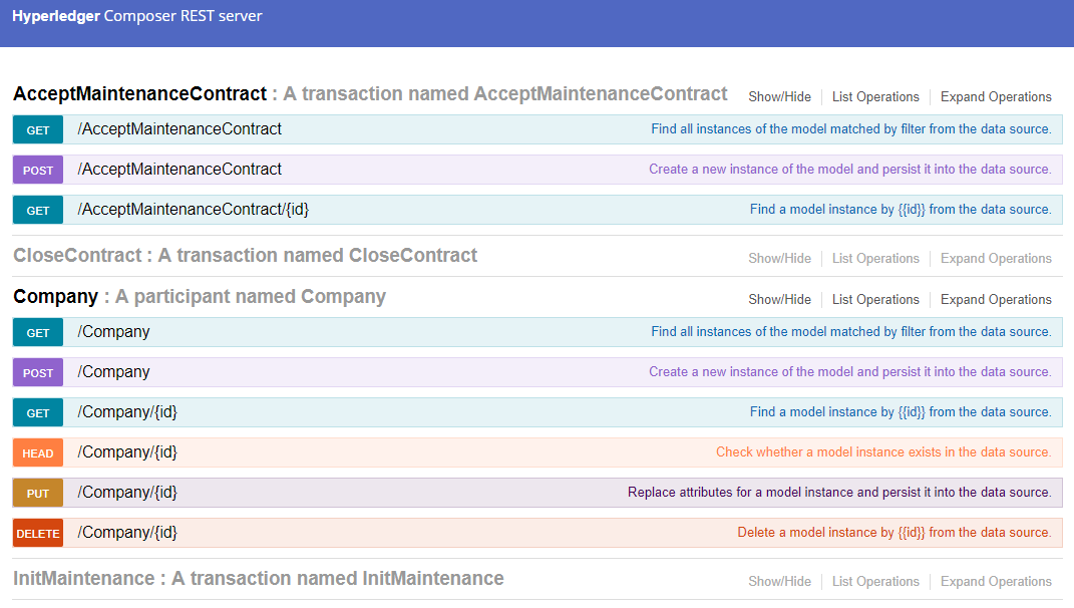
\includegraphics[width=1.0\textwidth,angle=0]{images/rest-api}
       \caption{Generierte REST-API zu der \acs{BND}. GET und POST Requests werden für Datenabfragen sowie das Ausführen von Transaktionen genutzt.}
      \label{fig:rest-api}
\end{figure}

\subsection{Webanwendungen}

\paragraph{Maintenance-App}

Die Maintenance-App ist eine Angular-Webanwendung. Mit ihr können Wartungsanbieter noch nicht angenommene Wartungsverträge einsehen und akzeptieren. Weiterhin kann das Loggen von Wartungsschritten sowie das Überprüfen der Vertragsschließung erfolgen. In der aktuellen Implementation ist der eingeloggte Nutzer durch den genutzten REST-Server definiert. Im Folgenden werden Codebeispiele zu den Abfragen und Erstellen von Assets sowie dem Abonnieren von Events gezeigt.

Listing \ref{lst:get-contracts} zeigt die Abfrage aller existierenden Wartungsverträge über einen GET-Request. Dieser wird über die in Zeile 2 angegebene URL an den REST-Server geschickt.

\begin{listing}[!htbp]
\begin{minted}
[
frame=lines,
fontsize=\footnotesize,
framesep=2mm,
breaklines,
linenos
]
{js}
public fetchAllContracts() : Observable<any> {
    let API_BASE = "http://10.40.94.180:12100/api/";
    return this.http.get(API_BASE + "MaintenanceContract");
}
\end{minted}
\caption{Abfrage aller existierenden Wartungsverträge.}
\label{lst:get-contracts}
\end{listing}

Es ist ebenfalls möglich GET-Requests mit Filtern auszuführen. Im Listing \ref{lst:get-contracts-filter} werden nur Wartungsverträge abgefragt, welche von den eingeloggten Wartungsanbieter akzeptiert, aber noch nicht geschlossen wurden. Die dazu in Zeile 5 entstandene URL wurde von der REST-Weboberfläche generiert. 

\begin{listing}[!htbp]
\begin{minted}
[
frame=lines,
fontsize=\footnotesize,
framesep=2mm,
breaklines,
breakafter=%
linenos
]
{js}
public getAcceptedContracts() : Observable<any> {
    let API_BASE = "http://10.40.94.180:12100/api/";
    let PROVIDERNAME = "Aintenance";

    return this.http.get(API_BASE + "MaintenanceContract?filter=%7B%22where%22%3A%7B%22and%22%3A%5B%7B%22isAccepted%22%3Atrue%7D%2C%7B%22isClosed%22%3Afalse%7D%2C%20%7B%22maintenanceProvider%22%3A%22resource%3Abiz.innovationcenter.maintenance.MaintenanceProvider%23" + PROVIDERNAME + "%22%7D%5D%7D%7D");
}
\end{minted}
\caption{Abfrage aller Wartungsverträge, welche vom eingeloggten Wartungsanbieter akzeptiert wurden und noch nicht geschlossen sind.}
\label{lst:get-contracts-filter}
\end{listing}

Zuletzt wird ein Beispiel zum Ausführen einer Transaktion gezeigt. Wartungsanbieter können über die \textit{AddPerformedStep}-Transaktion die durchgeführten Wartungsschritte loggen. Listing \ref{lst:post-transaction} zeigt den dafür auszuführenden POST-Request. In Zeile 2-6 wird ein JSON-Objekt erstellt, welches die auszuführende Transaktion sowie ihre Parameter festlegt. Dazu gehört der zu bearbeitende Vertrag sowie der ausgeführte Wartungschritt. Letztendlich wird das JSON-Objekt als Parameter der POST-Request übergeben und der im JavaScript-File der \acs{BND} angegebene Code der Transaktion ausgeführt.

\begin{listing}[!htbp]
\begin{minted}
[
frame=lines,
fontsize=\footnotesize,
framesep=2mm,
breaklines,
linenos
]
{js}
public addPerformedStep(operation : string, contractId : string) : Observable<any> {
    const body = {
        "$class": "biz.innovationcenter.maintenance.AddPerformedStep",
        "contract": contractId,
        "performedStep": operation
    };
    return this.http.post(API_BASE + 'AddPerformedStep', body);
}
\end{minted}
\caption{POST-Request zum Hinzufügen von durchgeführten Wartungsschritten zum Wartungsvertrag.}
\label{lst:post-transaction}
\end{listing}

\paragraph{Composer Playground}
Der Composer Playground ist eine in Composer enthaltene Webanwendung. Sie wird hauptsächtlich während der Entwicklung zum Testen der \acs{BND} verwendet wird. Über den Playground können Participants sowie Identitäten für diese erstellt werden. Ebenfalls ist es möglich, Assets zu erstellen und zu bearbeiten. Was die Anwendung jedoch auch für den Endnutzer attraktiv macht, ist, dass sie einen Überblick über alle bestehenden Daten gibt. Weiterhin ist es möglich Transaktionen ausführen und die Historie aller durchgeführten Transaktionen einzusehen. Es ist jedoch nicht möglich Daten zu filtern. Im bestehenden Prototypen soll der Playground hauptsächlich von den Unternehmen eingesetzt werden, um die Daten der Maschinen und Wartungsverträge einzusehen. Weiterhin muss er in der aktuellen Version von den Unternehmen und Wartungsanbietern genutzt werden, um die Preisabsprachen in der Blockchain zu dokumentieren. Bei einer Weiterentwicklung sollten dafür ebenfalls Webanwendungen entwickelt werden.

\subsection{XDK-Trigger}
Um die Simulation von Wartungsgeräten zu realisieren, wird ein Bosch Cross Domain Kit (XDK) genutzt. Dabei handelt es sich um ein Gerät mit diversen Sensoren. So misst es u. a. Temperatur, Luftfeuchtigkeit sowie Beschleunigung (bzw. G-Kräfte). Auf dem XDK ist ein Programm installiert, welches die Sensordaten über USB per Serial Port überträgt. Wenn bestimmte Daten angeliefert werden, sollen Transaktionen ausgeführt werden, um Wartungsverträge zu erstellen und zu schließen. Dafür wird eine Node.js-Anwendung geschrieben.

Ein Wartungsvertrag wird erstellt, sobald die Luftfeuchtigkeit einen bestimmten Schwellwert überschreitet. Das Schließen von Wartungsverträgen erfolgt, sobald das Gerät auf den Kopf gedreht wird. Dies würde das Drücken eines Knopfes an der zu wartenden Maschine simulieren, wodurch der Wartungsanbieter die fertige Wartung signalisiert sowie die Schließung des Vertrags beantragt. Damit die Transaktionen mit der Identität einer Maschine ausgeführt werden, muss ein dementsprechend konfigurierter REST-Server existieren. 

Listing \ref{lst:humidity-handling} zeigt, wie mit dem Überschreiten der Luftfeuchtigkeitsschwellwerts umgegangen wird. In Zeile 7 wird die Funktion \textit{createSmartContract} aufgerufen. Dieser führt die InitMaintenance-Transaktion über einen POST-Request aus. Dabei werden zufällige Werte für die Parameter \textit{contractId}, \textit{maintenanceReason} und \textit{lastRequiredStep} übergeben.

\begin{listing}[!htbp]
\begin{minted}
[
frame=lines,
fontsize=\footnotesize,
framesep=2mm,
breaklines,
linenos
]
{js}
function handleHumidityEvent() {
    var HUMIDITY_TRIGGER = 70;
    //If the humidity is too high, create a smart contract
    if (jsonData.humidity >= HUMIDITY_TRIGGER) {
        if (humidityFirstTimeExceeded) {
            //Execute InitMaintenance-Transaction via POST-Request
            console.log("HUMIDITY TOO HIGH! MY HAIR!!!");
            createSmartContract(); 
        }
        humidityFirstTimeExceeded = false;
    } else {
        humidityFirstTimeExceeded = true;
    }
}
\end{minted}
\caption{Erstellen eines Wartungsvertrags bei der Überschreitung des Schwellwerts für die Luftfeuchtigkeit.}
\label{lst:humidity-handling}
\end{listing}

\section{Netzwerkkonfiguration}
\label{sec:network-config}
Die Netzwerkkonfiguration besteht aus dem Erstellen einer Fabric-Netzwerk-Konfiguration sowie dem Konfigurieren von Composer zum Installieren der \acs{BND}. 

\subsection{Fabric-Netzwerk-Konfiguration}
Um das Blockchain-Netzwerk zu konfigurieren und zu starten, müssen Orderer Nodes, Peer Nodes, Certificate Authorities und Channel in mehreren Dateien definiert werden. Um diesen Prozess zu vereinfachen, wird das Tool \textit{netcomposer}\cite{IBMSilvergateTeamnetcomposerGithubRepository2018} genutzt. Dieses erstellt aus einem einzigen Konfigurationsfile alle benötigten Dateien, um ein Blockchain-Netzwerk zu starten. 

In dem zu erstellenden Netzwerk soll es zwei Unternehmen (Eiva und Twimbee), zwei Wartungsanbieter (Repairr und Aintenance), sowie zwei Maschinen (Server\_1 und Machine\_1), welche zu den Unternehmen gehören, geben (siehe Abb. \ref{fig:architecture-high}). Eine verkürzte Konfiguration dafür ist im Listing \ref{lst:network-config} angegeben. In Zeile 1 wird der genutzte Konsensmechanismus angegeben. In der aktuellen Implementation gibt es nur eine Ordering Node. Der Grund dafür wird genauer im Kapitel \ref{sec:consensus-choose} erläutert. In Zeile 4 wird die für die State Database zu nutzende Datenbank definiert. Von Zeile 10-21 werden die Channels konfiguriert. Der Channel \textit{mychannel} ist der öffentliche Channel, während \textit{privatechannel} nur zwischen 2 Organisationen besteht. 

\begin{figure}[!htbp]
    \centering
      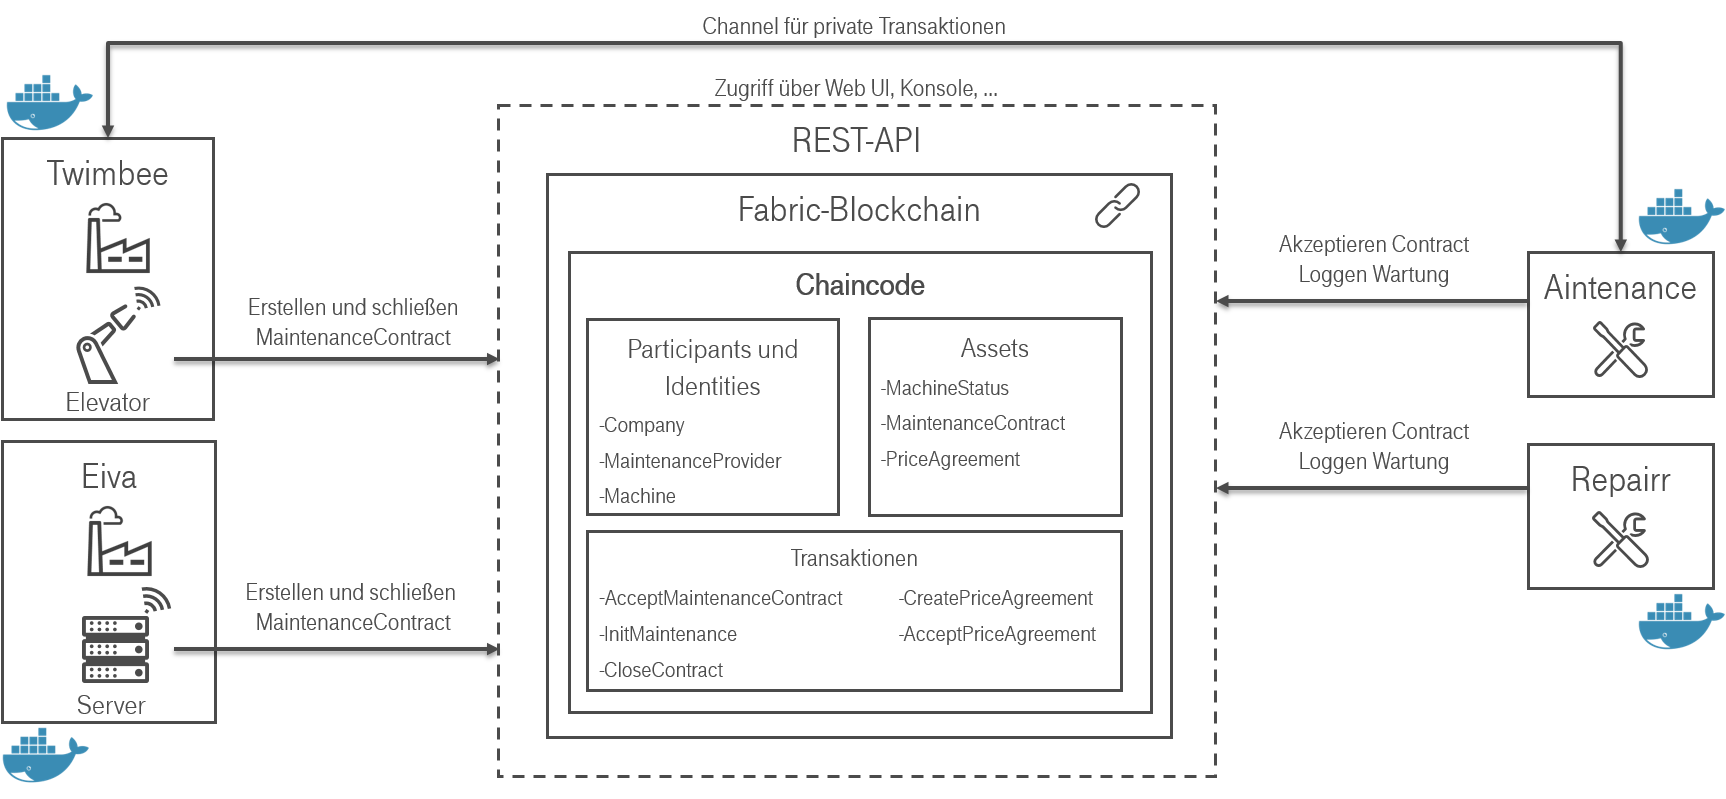
\includegraphics[width=1.0\textwidth,angle=0]{images/architecture_highlevel}
       \caption{High-Level-Architektur des zu entstehenden Fabric-Netzwerks.}
      \label{fig:architecture-high}
\end{figure}

\begin{listing}[!htbp]
\begin{minted}
[
frame=lines,
fontsize=\footnotesize,
framesep=2mm,
breaklines,
linenos
]
{yaml}
orderer:
    type: "solo"
db:
    provider: "CouchDB"

organizations:      4
peersPerOrganization:   1
usersPerOrganization:   1

channels:
    - name: mychannel
        organizations:
        - organization: 1
        - organization: 2
        - organization: 3
        - organization: 4

    - name: privatechannel
        organizations:
        - organization: 1
        - organization: 2
\end{minted}
\caption{Konfiguration des Fabric-Netzwerks (verkürzt).}
\label{lst:network-config}
\end{listing}


Aus diesem Konfigurationsfile werden verschiedene Dateien generiert, u. a. auch ein Docker-Compose-File. Fabric nutzt Docker-Container\footnote{Docker-Container: Virtualisiertes Abbild, welches eine Applikation und alle Ressourcen zur Ausführung dieser beinhaltet \cite{DockerTeamWhatcontainer2017}.}, um die Peer Nodes, Ordering Nodes, State Databases und Certificate Authorities zur Verfügung zu stellen. Das Docker-Compose-File wird genutzt, um die im Konfigurationsfile angegebenen Komponenten zu starten. Nach dem Start der Container muss die Kommandozeile genutzt werden, um die Channel zu starten und die Peers diesen hinzuzufügen. Dies erfolgt letztendlich über selbst erstellte Shell-Skripte. 


\subsection{Composer-Konfiguration}
Um die \acs{BND} zu installieren, müssen Connection Profiles erstellt werden. Über diese wird Composer u. a. mit den IP-Adressen der Peers bekannt gemacht. In der genutzten Version von Composer müssen für jede Organisation je Channel 2 Profile erstellt werden. Anschließend müssen über die Kommandozeile Identitäten beantragt werden, über welche die Installation der \acs{BND} erfolgt. Ebenfalls werden Identitäten erstellt, welche die Admins der \acs{BND} der einzelnen Organisationen darstellen. Letztendlich wird die \textit{SetupDemo}-Transaktion ausgeführt, um die Beispieldaten zu erstellen. Im Zuge dessen werden auch Identitäten für die Maschinen erstellt. Der Prozess erfolgt über selbst erstellte Shell-Skripte. Der gesamte Vorgang ist im Detail genauer unter \cite{HyperledgerComposerTeamMultiOrgDeployment} beschrieben.

\section{Konsensmechanismus}
\label{sec:consensus-choose}
Kapitel \ref{sec:eval-konsens} beschreibt verschiedene Konsensmechanismen. Für den Use-Case empfiehlt sich die Nutzung des \acs{PBFT}. Dieser erlaubt bei der Teilnehmerzahl von 4 Nodes einen Transaktionsdurchsatz von mehr als 14000 \acs{TPS}. Weiterhin werden bis zu \nicefrac{1}{3} an unvertrauenswürdigen Nodes toleriert. Der \acs{PBFT} ist allerdings noch nicht Out-of-the-box in Fabric implementiert. Dies soll in Zukunft jedoch noch erfolgen \cite{HyperledgerFabricTeamPluggableConsensusImplementations}. Für den Prototypen müsste also eine Implementation des \acs{PBFT} manuell erfolgen. Aufgrund des Zeitaufwands erfolgt dies im Rahmen der Prototyp-Entwicklung nicht. Fabric implementiert aktuell nur einen Konsensmechanismus basierend auf Apache Kafka\footnote{Apache Kafka: Plattform zur Verarbeitung von Datenströmen \cite{ApacheIntroductionApacheKafka}.}. Dieser ist jedoch unsicher, da keine unvertrauenswürdigen Nodes toleriert werden. Genauere Informationen können \cite{CachinBlockchainConsensusProtocols2017} entnommen werden.

\section{Showcase-Demo}
Letztendlich wird für den Prototypen eine Demo entworfen. Diese demonstriert die Funktionsweise sowie diverse Workflows der Anwendung. Die Komponenten der Demo werden in Abbildung \ref{fig:architecture-showcase} visualisiert. Alle Komponenten können innerhalb der genannten Entwicklungsumgebung oder auf einer beliebigen Ubuntu-Umgebung laufen. Das Unternehmen Twimbee, welches einen Server besitzt, ist eine Node des Netzwerks. Auf dieser Node läuft ebenfalls ein REST-Server, über welchen der Server Wartungsverträge auf der (lokal laufenden) Blockchain erstellen kann. Weiterhin nutzt Twimbee den Playground, um Daten auf der öffentlichen sowie privaten Blockchain einzusehen. Auf den privaten Channel werden über den Playground ebenfalls Preisabsprachen dokumentiert. Der Wartungsanbieter Aintenance ist ähnlich aufgebaut. Der einzige Unterschied besteht darin, dass Aintenance anstatt eines Servers, eine lokale Webapplikation besitzt, welche mit seinen REST-Server kommuniziert. Eine noch nicht erwähnte Applikation ist der Hyperledger Blockchain Explorer \cite{HyperledgerBlockchainExplorerTeamHyperledgerBlockchainExplorer2018}. Über ihn erfolgt die Einsicht und Visualisierung der Rohdaten auf der Blockchain. Die Anwendung kann ebenfalls bei jeden Teilnehmer selbst bereitgestellt sein.

\begin{figure}[!htbp]
    \centering
      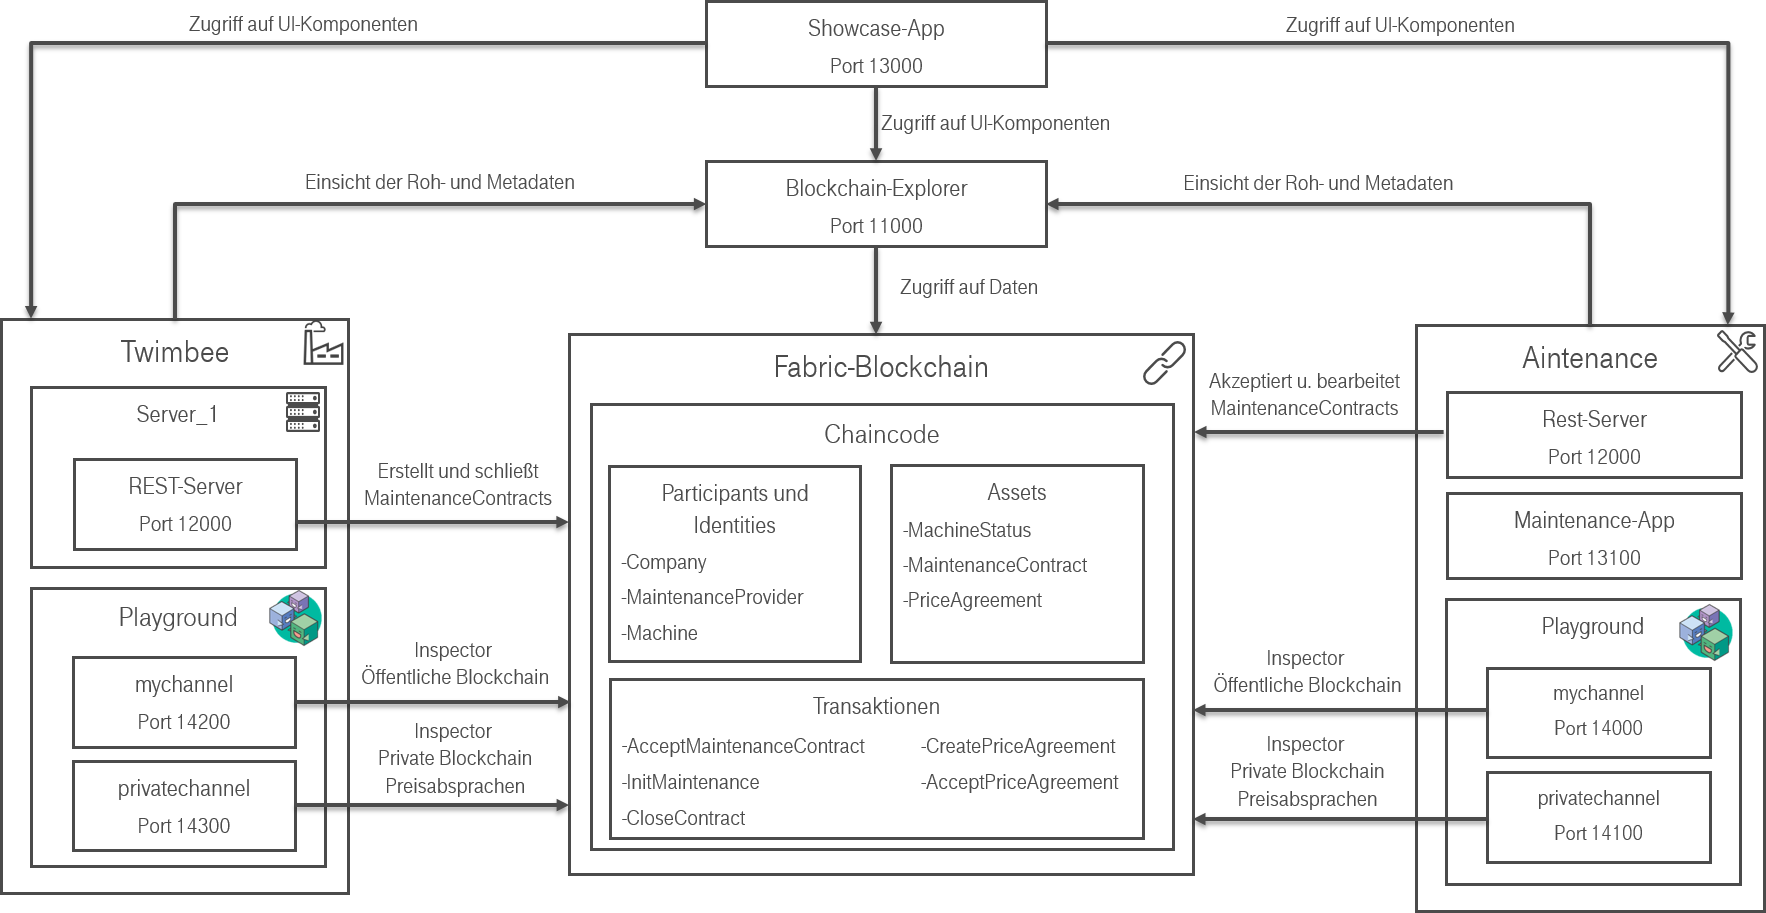
\includegraphics[width=1.0\textwidth,angle=0]{images/architecture_showcase}
       \caption{Architektur der Demo-Komponenten.}
      \label{fig:architecture-showcase}
\end{figure}

In der Demo wird der Workflow des Sequenzdiagramms der Abbildung \ref{fig:maintenance-workflow} demonstriert. Es beschreibt den Workflow für die Wartung eines Geräts. Zunächst wird die Webapplikation der Wartungsanbieter geöffnet. Der Bosch XDK wird angehaucht, um den Schwellwert für die Luftfeuchtigkeit zu überschreiten. Anschließend wird vom ihm die \textit{InitMaintenance}-Transaktion über den REST-Server aufgerufen und somit ein Wartungsvertrag erstellt. Dieser Wartungsvertrag erscheint daraufhin in der Webapplikation der Wartungsanbieter und wird angenommen. Danach werden verschiedene Wartungsschritte geloggt, inklusive des letzten geforderten Schrittes. Die eingetragenen Schritte werden in der Webapplikation sichtbar. Letztendlich wird der Bosch XDK auf den Kopf gedreht, wodurch die Schließung des Vertrags beantragt wird. Ist der letzte erforderliche Wartungsschritt in der Blockchain eingetragen, ist dies erfolgreich.

\begin{figure}[!htbp]
    \centering
      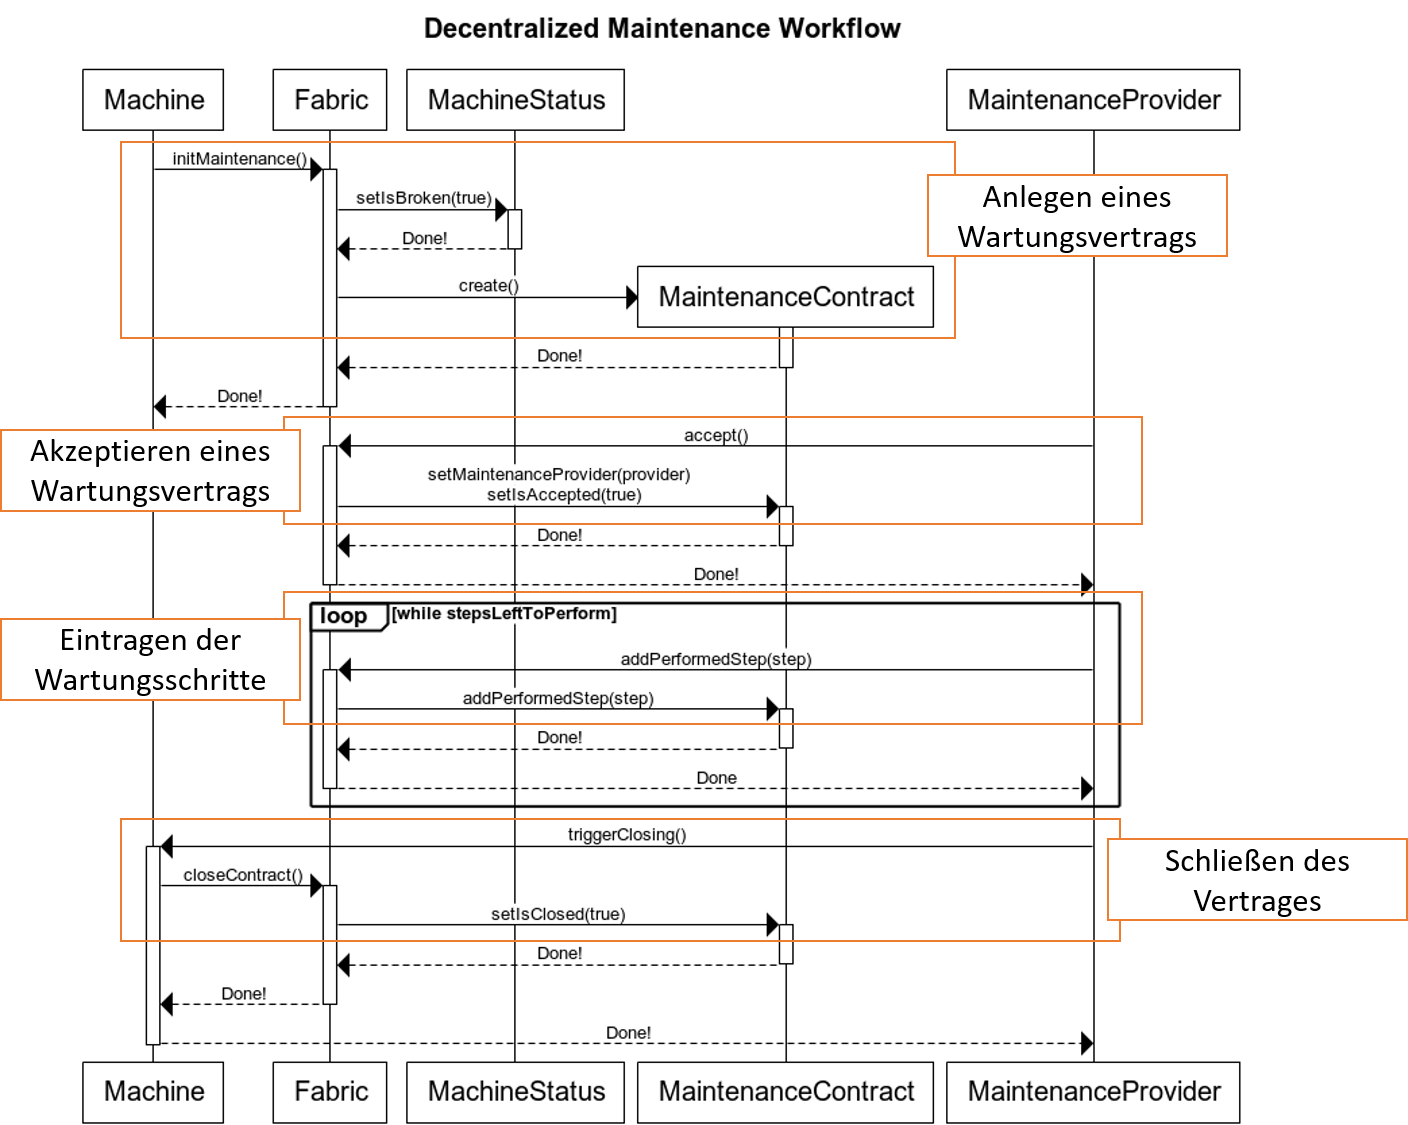
\includegraphics[width=1.0\textwidth,angle=0]{images/maintenance-workflow-marked}
       \caption{Workflow für die Wartung.}
      \label{fig:maintenance-workflow}
\end{figure}

Anschließend wird kurz der Playground für die Dateneinsicht vorgestellt. In Zuge dessen wird gezeigt, dass es möglich ist, den Playground auf den öffentlichen und privaten Channel zu nutzen. Um die Funktion des privaten Channels zu zeigen, wird eine Preisabsprache von Twimbee erstellt. Wenn der Wartungsanbieter mit dieser einverstanden ist, kann er sie akzeptieren. Anschließend wird gezeigt, dass die Preisabsprache nicht im öffentlichen Channel vorkommt.

In der Demo erfolgt als letztes die Demonstration des Blockchain Explorer. Über ihn kann u. a. die Anzahl der bestehenden Blöcke und Peers sowie die Details der Transaktionen eingesehen werden.
\chapter{Fazit und Ausblick}
\label{cha:fazit}

Die Blockchain-Technologie hat das Potenzial, dezentrale Anwendungen zu ermöglichen, in welchen Transaktionen nicht manipuliert oder gelöscht werden können. Öffentliche Blockchains bringen jedoch noch Probleme bezüglich Skalierbarkeit und Privatsphäre mit sich. Permissioned Blockchains können diese Probleme zu Teilen lösen, nehmen dafür aber eine stärkere Zentralisierung und weniger sichere Konsensmechanismen in Kauf. 

Es wurde ein Proof-of-Concept für einen dezentralen Wartungsmarkt entwickelt. Die Implementation von diesem mit der Blockchain bringt verschiedene Vorteile gegenüber klassischen B2B-Anwendungen mit sich. Die Teilnehmer müssen keiner zentral verwaltenden Instanz vertrauen und können ihre Daten trotzdem an einer einheitlichen Stelle zur Verfügung stellen. Es gilt jedoch noch verschiedene Dinge zu bedenken, Limitationen zu untersuchen und Funktionen zu verbessern. Aktuell kann keine eindeutige Aussage zu der Skalierbarkeit und Performance getroffen werden. Der maximal mögliche Transaktionsdurchsatz von Hyperledger Fabric müsste mit leistungsstärkeren Systemen untersucht werden, um eine Aussage darüber zu treffen, ob ein Wartungsmarkt mit mehreren tausend Teilnehmern und Maschinen bestehen kann. Diesbezüglich muss ebenfalls eine Analyse des \acs{PBFT} erfolgen, wenn es mehr als 64 Nodes gibt. Ebenfalls besteht die Frage, ob es für B2B-Anwendungen ausreichend ist, wenn \nicefrac{1}{3} an nicht vertrauenswürdigen Teilnehmern toleriert werden. Deshalb ist es wichtig, dass weitere Analysen von Hyperledger Fabric in der Zukunft erfolgen. Letztendlich steht fest, dass die Performance mit der Anzahl an Nutzern sinkt und Anwendungen deswegen auf einen bestimmten Transaktionsdurchsatz bzw. auf eine bestimmte Anzahl an Peer-Nodes beschränkt sind. 

Der entwickelte dezentrale Wartungsmarkt beinhaltet nur Features, welche für einen Proof-of-Concept benötigt werden. Er kann in diversen Bereichen erweitert werden. So können beispielsweise Remote-Support-Verträge eingeführt werden. Die Wartungsanbieter könnten, falls sie mit der Wartung keinen Erfolg haben, Hilfe über ihr Smartphone oder ihre Smart Glasses anfordern. Experten, welche Teilnehmer an der Blockchain sind, würden dann beispielsweise über ein Videogespräch den Support leisten. Ein weiteres interessantes Konzept ist ein Reputation System. Heutige Bewertungssysteme haben das Problem, dass falsche Bewertungen abgegeben werden, beispielsweise um Nutzer zu schädigen. Die Bewertung der Wartungsanbieter könnte jedoch automatisch über in der Blockchain bestehende Daten, wie zum Beispiel die benötigte Zeit für eine Wartung, erfolgen. Solche Systeme werden ebenfalls in den Arbeiten von Carboni \cite{CarboniFeedbackbasedReputation2015} und Dennis \cite{DennisRepblocknext2015} vorgestellt.

Ebenfalls bringen Hyperledger Fabric und Composer selbst Probleme mit sich. Die Konfiguration eines Netzwerks ist mit sehr viel Aufwand verbunden. Um im aktuellen Prototyp neue Teilnehmer hinzuzufügen, muss eine neue Konfiguration erstellt werden, wodurch auch alle davon abhängigen Shell-Skripte bearbeitet werden müssen. Ebenfalls gibt es nur einen mitgelieferten, nutzbaren Konsensmechanismus. Andere, wie PBFT, müssten selbst implementiert werden, was zusätzlichen Aufwand bedeutet. Das fehlende Data Sharing zwischen Channeln kann ebenfalls problematisch sein. Es ist nicht möglich, Daten vom Public Channel mit dem Private Channel zu teilen. So können private Transaktionen keine Referenz zu einem im Public Channel bestehenden Asset herstellen.

Ein letzter Punkt, welcher in Bezug zu Blockchain-Anwendungen erwähnt werden muss, ist, dass die Blockchain keine Korrektheit der Daten garantiert. So sagen beispielsweise Wüst et al., dass ``das Interface zwischen physischer und digitaler Welt'' ein Problem darstellt \cite{WustyouneedBlockchain2017}. So könnte beispielsweise beim Prototyp ein Wartungsanbieter durchgeführte Wartungsschritte dokumentieren, welche gar nicht erfolgt sind. Um dies zu lösen, könnte ein Sensor anhand verschiedener Daten überprüfen, ob ein Wartungsschritt erfolgt ist. Dann muss allerdings diesen vertraut werden. Um Wartungsanbieter zu schädigen, könnte der Sensor vom Unternehmen manipuliert worden sein. Letztendlich garantiert die Blockchain nur, dass eingetragene Daten bzw. ausgeführte Transaktionen nicht manipulier- und löschbar sind sowie bei allen Teilnehmern gleich vorkommen. Um falschen Input zu verhindern, müssen andere Lösungen gefunden werden.

Auch wenn es noch Fragen zu klären gilt, zeigt der entwickelte Wartungsmarkt die Machbarkeit von Blockchain-Anwendungen für B2B. Die Probleme der Technologie sowie der Nutzen von Permissioned Blockchains müssen weiterhin untersucht werden. Ebenfalls ist wichtig, dass mehr Blockchain-Anwendungen entwickelt und eingesetzt werden. So werden die sinnvollen Use-Cases ergründet und die Technologie besser verstanden. Nur so kann sich die Blockchain im B2B-Bereich etablieren.







%----------------- KAPITEL : BEISPIELE  ----------------- %	
% \chapter{Beispiele}
% \label{cha:beispiele}
% 	Dieses Kapitel soll viele alltaegliche Beispiele\footnote{Fussnote} abdecken um einen {\LaTeX} Dokument zu setzen \cite{WustyouneedBlockchain2017}

% 		\section{Schriftarten}
% 		\label{sec:schriftarten} 
% 			\begin{itemize}
% 				\item Kursiv: \emph{Das ist ein Beispiel}
% 				\item Unterstreichen: \underline{Das ist ein Beispiel}
% 				\item Fettschrift: \textbf{Das ist ein Beispiel}
% 				\begin{itemize} 
% 					\item Kombination aus dreien: \underline{\textbf{\emph{Das ist ein Beispiel}}}						\end{itemize} 
% 				\item Serifen: \textsf{Das ist ein Beispiel}
% 				\item Schreibmaschinen Schrift: \texttt{Das ist ein Beispiel}
% 				\item Kleine Grossbuchstassen: \textsc{Das ist ein Beispiel}
% 				\item Ausfuehrungszeichen: ``Das ist ein Beispiel''
% 				\item asld
% 			\end{itemize}
			
		
			
				

% 	\section{Abbildungen}
% 		Wie folgt bindet man Abbildungen ein:
% 		% Beispiel für Bildintegration
% 		\begin{figure}[!htbp]
% 		 \centering
% 		 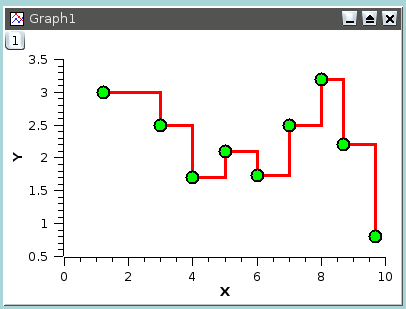
\includegraphics[width=0.4\textwidth,angle=0]{images/beispiel}
%  		\caption{Beispiel Bild; Quelle ist png}
% 		\label{fig:beispiel}
% 		\end{figure}
	
% 	\section{Tabellen}
% 			Lorem ipsum dolor sit amet, consetetur sadipscing elitr, sed diam nonumy eirmod tempor invidunt ut labore et dolore magna aliquyam erat, sed diam voluptua. At vero eos et accusam et justo duo dolores et ea rebum. Stet clita kasd gubergren.

% 		\begin{center}
% 			\begin{tabular}{lcrc} \toprule
% 			Stadium & Substratfreie Kontrolle  & \multicolumn{2}{c}{Probenansatz} \\\cmidrule(rl){3-4}
% 			 & Farbe & Farbe & Bewertung \\\midrule
% 			Alpha1 & farblos & braun & +++ \\
% 			Beta2 & farblos & farblos & - \\\bottomrule 
% 			 \end{tabular}
% 		 \end{center}
		 
% 		2. Beispiel \\
% 		\begin{table}[h]
% 		\centering	 
% 		 	\begin{tabular}{|l|l|c|}
% 			\hline
% 			\textsc{Rang} & \textsc{Name} & \textsc{Rating}\\
% 			\hline
% 			\hline
% 			1 & Garry Kasparov & 2817\\
% 			2 & Viswanathan Anand & 2774\\
% 			3 & Wladimir Kramnik & 2764\\
% 			\hline
% 			\end{tabular}
% 		\caption{Beispiel Beschriftung einer Tabelle}
% 		\label{tab:beispiel}
% 		\end{table}
		
		


% 	\section{Verweise}
% 		Hier werden Verweise auf verschiedene Elemente erstellt.
% 		\subsection{Pageref und Ref} 
% 			Diese Textstelle ist sehr interessant.\label{interessant} \\				
% 			Hier wird auf die Textstelle~\ref{interessant} verwiesen, \\
% 			die sich auf der Seite~\pageref{interessant} befindet.\\[20pt] 
% 			Verweis auf Listing \ref{lst:javaBsp} auf Seite \pageref{lst:javaBsp} \\
% 			Verweis auf Abbildung \ref{fig:beispiel} auf Seite \pageref{fig:beispiel} \\
% 			Verweis auf Tabelle \ref{tab:beispiel} auf Seite \pageref{tab:beispiel}
			
% 	\section{Listing}
% 		\lstset{language=java}
% 		\begin{lstlisting}[frame=hl, caption={Das Listing zeigt Java Quellcode} ,backgroundcolor=\color{gray}, label={lst:javaBsp}]
% /* Java Hallo World Beispiel */

% public class HelloWorld {
%     public static void main(String[] args) {
%         System.out.println("Hello, World");
%     }
% }
% 		\end{lstlisting} 
		
    
%\bibliographystyle{plain}
%\bibliography{literature}	
\printbibliography

\begin{appendices}

\chapter{Composer BNA: Model-File}
\label{append:model-file}
    
\begin{lstlisting}[frame=hl, caption={Composer BNA Model-File} ,backgroundcolor=\color{gray}]
namespace biz.innovationcenter.maintenance

participant Company identified by companyName {
o String companyName  
}

participant Machine identified by machineId {
o String machineId
o String type
o String model
--> Company owner
}

participant MaintenanceProvider identified by companyName {
o String companyName
o String experienceWith
}

asset MachineStatus identified by machineStatusId {
o String machineStatusId
o Boolean isBroken
--> Machine owner
}

asset MaintenanceContract identified by maintenanceContractId {
o String maintenanceContractId
o String maintenanceReason
o Boolean isAccepted
o Boolean isClosed
o String[] performedSteps
o String requiredLastStep optional
--> Machine owner
--> MaintenanceProvider maintenanceProvider optional
}

asset PaymentAgreement identified by paymentAgreementId {
o String paymentAgreementId
o Integer payment
o String maintenanceContractId
o Boolean isAccepted
}

transaction AcceptMaintenanceContract {
--> MaintenanceContract maintenanceContract
}

transaction InitMaintenance {
o Integer contractId
o String requiredLastStep optional
o String maintenanceReason optional
}

transaction CloseContract {
--> MaintenanceContract contract
}

transaction AddPerformedStep {
--> MaintenanceContract contract
o String performedStep
}

transaction AcceptPaymentAgreement {
--> PaymentAgreement paymentAgreement
}

transaction CreatePaymentAgreement {
o Integer paymentAgreementId
o Integer payment
o String maintenanceContractId
}

transaction SetupDemo {
}

event NewContractCreated {
}

event ContractClosed {
--> MaintenanceContract contract
--> MaintenanceProvider provider
}
\end{lstlisting}

\chapter{Composer BNA: JavaScript-File}
\label{append:javascript-file}

\begin{lstlisting}[frame=hl, caption={Composer BNA JavaScript File} ,backgroundcolor=\color{gray}]
'use strict';
/**
    * Write your transction processor functions here
    */

var NAMESPACE = 'biz.innovationcenter.maintenance';
var MACHINE_STATUS_SUFFIX = '_Status';
var MAINTENANCE_CONTRACT_SUFFIX = '_Contract';
var PAYMENT_AGREEMENT_PREFIX = 'Agreement_';

/**
    * Accept the MaintenanceContract
    * @param {biz.innovationcenter.maintenance.AcceptMaintenanceContract} tx The transaction instance.
    * @transaction
    */
function acceptMaintenanceContract(tx) {
    var error = null;

    //Check if the contract is already accepted
    if (tx.maintenanceContract.isAccepted === false) {
        //Check if the Participant has the required experience
        if (tx.maintenanceContract.owner.type === getCurrentParticipant().experienceWith) {
            //Set the new Contract Data
            tx.maintenanceContract.isAccepted = true;
            tx.maintenanceContract.maintenanceProvider = getCurrentParticipant();

            // Get the contract from the asset registry
            return getAssetRegistry('biz.innovationcenter.maintenance.MaintenanceContract')
                .then(function (assetRegistry) {
                    // Update the contract the asset registry.
                    return assetRegistry.update(tx.maintenanceContract);
                });
        } else {
            error = 'Error: Provider does not have required experience';
        }
    } else {
        error = 'Error: Contract is already accepted';
    }

    if (error !== null) {
        console.error(error);
        throw error;
    }
}

/**
    * Initiate the maintenance. Set status to broken and create a maintenance contract.  Can only be executed by machines(see ACL).
    * @param {biz.innovationcenter.maintenance.InitMaintenance} tx The transaction instance.
    * @transaction
    */
function initMaintenance(tx) {
    //TODO: Add condition
    var factory = getFactory();

    console.log('initMaintenance');
    var machineId = getCurrentParticipant().getIdentifier()
    var machineStatusId = machineId + MACHINE_STATUS_SUFFIX;
    console.log("CURRENT MACHINE STATUS ID: " + machineStatusId);

    //Initiate the MaintenanceContract
    var contractName = machineId + MAINTENANCE_CONTRACT_SUFFIX + "_" + tx.contractId;
    var contract = factory.newResource(NAMESPACE, 'MaintenanceContract', contractName);
    if (tx.maintenanceReason != undefined) {
        contract.maintenanceReason = tx.maintenanceReason;
    }
    else {
        contract.maintenanceReason = "Unknown";
    }

    if (tx.requiredLastStep != undefined) {
        contract.requiredLastStep = tx.requiredLastStep;
    }
    else {
        contract.requiredLastStep = "Unknown";
    }    
    contract.isAccepted = false;
    contract.isClosed = false;
    contract.performedSteps = [];
    
    contract.owner = factory.newRelationship(NAMESPACE, 'Machine', machineId);

    //Update the MachineStatus
    return getAssetRegistry(NAMESPACE + '.MachineStatus')
        .then(function (machineStatusRegistry) {
            return machineStatusRegistry.get(machineStatusId)
                .then(function (machineStatus) {
                    machineStatus.isBroken = true;
                    return machineStatusRegistry.update(machineStatus);
                })
        })
        //Add the contract to the registry
        .then(function () {
            return getAssetRegistry(NAMESPACE + '.MaintenanceContract')
                .then(function (contractRegistry) {
                    return contractRegistry.add(contract);
                })
                .then(function() {
                    //Emit event
                    var factory = getFactory();
                    var newContractEvent = factory.newEvent(NAMESPACE, 'NewContractCreated');
                    emit(newContractEvent);
                });
        });

}

/**
    * Add a performed maintenance step to the contract
    * @param {biz.innovationcenter.maintenance.AddPerformedStep} tx The transaction instance.
    * @transaction
    */
function addPerformedStep(tx) {
    //Update contract
    if (tx.contract.isAccepted == true) {
        if (tx.performedStep != "") {
            tx.contract.performedSteps.push(tx.performedStep);
            return getAssetRegistry(NAMESPACE + '.MaintenanceContract')
                .then(function (contractRegistry) {
                    return contractRegistry.update(tx.contract);
                });
        }

    } else {
        var error = 'Error: Contract is not accepted';
        console.error(error);
        throw error;
    }
}

/**
    * Close the given Contract
    * @param {biz.innovationcenter.maintenance.CloseContract} tx The transaction instance.
    * @transaction
    */
function closeContract(tx) {
    //Update contract
    if (tx.contract.isAccepted == true) {
        if (tx.contract.performedSteps.length != 0) {
            if (tx.contract.requiredLastStep == "Unknown" || tx.contract.requiredLastStep == tx.contract.performedSteps[tx.contract.performedSteps.length - 1]) {
                tx.contract.isClosed = true;
                return getAssetRegistry(NAMESPACE + '.MaintenanceContract')
                    .then(function (contractRegistry) {
                        return contractRegistry.update(tx.contract);
                    })
                    .then(function () {
                        console.log("Getting machine status registry");
                        return getAssetRegistry(NAMESPACE + '.MachineStatus')
                            .then(function (machineStatusRegistry) {
                                machineStatusRegistry.get(tx.contract.owner.getIdentifier() + MACHINE_STATUS_SUFFIX)
                                    .then(function (machineStatus) {
                                        //Update contract
                                        machineStatus.isBroken = false;
                                        return machineStatusRegistry.update(machineStatus);
                                    })
                                    .then(function() {
                                        //Emit event
                                        var factory = getFactory();
                                        var contractClosedEvent = factory.newEvent(NAMESPACE, 'ContractClosed');
                                        contractClosedEvent.contract = tx.contract;
                                        contractClosedEvent.provider = tx.contract.maintenanceProvider;
                                        emit(contractClosedEvent);
                                    });
                            });
                    });
            } else {
                var error = 'Error: Required last step was not performed';
                console.error(error);
                throw error;
            }
        } else {
            error = 'Error: No steps performed';
            console.error(error);
            throw error;
        }
    } else {
        error = 'Error: Contract is not accepted';
        console.error(error);
        throw error;
    }
}

/**
    * Add a performed maintenance step to the contract
    * @param {biz.innovationcenter.maintenance.CreatePaymentAgreement} tx The transaction instance.
    * @transaction
    */
function createPaymentAgreement(tx) {
    var factory = getFactory();
    var agreement = factory.newResource(NAMESPACE, 'PaymentAgreement', PAYMENT_AGREEMENT_PREFIX + tx.paymentAgreementId);    
    agreement.payment = tx.payment;
    agreement.maintenanceContractId = tx.maintenanceContractId;
    agreement.isAccepted = false;

    return getAssetRegistry(NAMESPACE + '.PaymentAgreement')
        .then(function (agreementRegistry) {
            return agreementRegistry.add(agreement);
        });
}

/**
    * Add a performed maintenance step to the contract
    * @param {biz.innovationcenter.maintenance.AcceptPaymentAgreement} tx The transaction instance.
    * @transaction
    */
function acceptPaymentAgreement(tx) {
    tx.paymentAgreement.isAccepted = true;

    return getAssetRegistry(NAMESPACE + '.PaymentAgreement')
        .then(function (agreementRegistry) {
            return agreementRegistry.update(tx.paymentAgreement);
        });
}

/**
    * Setup the demo
    * @param {biz.innovationcenter.maintenance.SetupDemo} setupDemo - the SetupDemo transaction
    * @transaction
    */
function setupDemo(setupDemo) {
    console.log('setupDemo');

    var factory = getFactory();

    //Declare the existing participants and assets
    var companyNames = ['Twimbee', 'Eiva'];
    var maintenanceProvNames = ['Repairr', 'Aintenance'];
    var machineNames = ['Elevator_1', 'Server_1'];
    var machineTypes = ['Elevator', 'Server'];
    var machineModels = ['EL213', 'SRV4'];

    //Create the resources and add them to arrays
    var companies = [];
    var maintenanceProviders = [];
    var machines = [];
    var machineStatuses = [];

    for (var i in companyNames) {
        var name = companyNames[i];
        var company = factory.newResource(NAMESPACE, 'Company', name);
        companies.push(company);
    }

    for (var i in maintenanceProvNames) {
        var name = maintenanceProvNames[i];
        var provider = factory.newResource(NAMESPACE, 'MaintenanceProvider', name);
        provider.experienceWith = machineTypes[i];
        maintenanceProviders.push(provider);
    }

    var i = 0;
    for (var i in machineNames) {
        var name = machineNames[i]
        var machine = factory.newResource(NAMESPACE, 'Machine', name);
        machine.type = machineTypes[i];
        machine.model = machineModels[i];
        machine.owner = factory.newRelationship(NAMESPACE, 'Company', companies[i].companyName)
        machines.push(machine);
        i++;
    }

    var i = 0;
    for (var i in machines) {
        var name = machineNames[i] + MACHINE_STATUS_SUFFIX;
        console.log("MACHINE NAME: " + name);
        var machineStatus = factory.newResource(NAMESPACE, 'MachineStatus', name);
        machineStatus.isBroken = false;
        machineStatus.owner = factory.newRelationship(NAMESPACE, 'Machine', machineNames[i]);
        machineStatuses.push(machineStatus);
        i++;
    }

    //Update the registries
    return getParticipantRegistry(NAMESPACE + '.Company')
        .then(function (companyRegistry) {
            return companyRegistry.addAll(companies);
        })
        .then(function () {
            return getParticipantRegistry(NAMESPACE + '.MaintenanceProvider');
        })
        .then(function (machineProvRegistry) {
            return machineProvRegistry.addAll(maintenanceProviders);
        })
        .then(function () {
            return getParticipantRegistry(NAMESPACE + '.Machine');
        })
        .then(function (machineRegistry) {
            return machineRegistry.addAll(machines);
        })
        .then(function () {
            return getAssetRegistry(NAMESPACE + '.MachineStatus');
        })
        .then(function (machineStatusRegistry) {
            return machineStatusRegistry.addAll(machineStatuses);
        });
}
\end{lstlisting}

\chapter{Composer BNA: ACL-Rules}
\label{append:acl-rules}

\begin{lstlisting}[frame=hl, caption={Composer BNA ACL-Rules} ,backgroundcolor=\color{gray}]
rule NetworkAdminUser {
    description: "Grant business network administrators full access to user resources"
    participant: "org.hyperledger.composer.system.NetworkAdmin"
    operation: ALL
    resource: "**"
    action: ALLOW
}

rule NetworkAdminSystem {
    description: "Grant business network administrators full access to system resources"
    participant: "org.hyperledger.composer.system.NetworkAdmin"
    operation: ALL
    resource: "org.hyperledger.composer.system.**"
    action: ALLOW
}

rule CompanyCanCreateMachineParticipants {
    description: "Allow companies to create machine-participants"
    participant(p): "biz.innovationcenter.maintenance.Company"
    operation: CREATE
    resource(m): "org.hyperledger.composer.system.Participant"
    condition: (p.getIdentifier() == m.owner.getIdentifier())
    action: ALLOW
}

rule CompanyCanDeleteMachineParticipants {
    description: "Allow companies to delete own machine-participants"
    participant(p): "biz.innovationcenter.maintenance.Company"
    operation: DELETE
    resource(m): "org.hyperledger.composer.system.Participant"
    condition: (p.getIdentifier() == m.owner.getIdentifier())
    action: ALLOW
}

rule MachineCanCreateStatusAsset {
    description: "Machine can create own Status-Asset"
    participant(p): "biz.innovationcenter.maintenance.Machine"
    operation: CREATE
    resource(m): "biz.innovationcenter.maintenance.MachineStatus"
    condition: ((p.getIdentifier() == m.owner.getIdentifier()) && (m.isBroken == false))
    action: ALLOW
}

rule MachineCanUpdateStatusAsset {
    description: "Machine can update own status-asset"
    participant: "biz.innovationcenter.maintenance.Machine"
    operation: UPDATE
    resource: "biz.innovationcenter.maintenance.MachineStatus"
    action: ALLOW
}

rule MachineCanCreateAndUpdateMaintenanceContract {
    description: "Machine can create and update MaintenanceContract-Asset"
    participant(p): "biz.innovationcenter.maintenance.Machine"
    operation: CREATE, UPDATE
    resource(m): "biz.innovationcenter.maintenance.MaintenanceContract"
    condition: (p.getIdentifier() == m.owner.getIdentifier())
    action: ALLOW
}

rule MaintenanceProviderCanUpdateMaintenanceContract {
    description: "Maintenance provider can update his accepted maintenanceContract"
    participant(p): "biz.innovationcenter.maintenance.MaintenanceProvider"
    operation: UPDATE
    resource(r): "biz.innovationcenter.maintenance.MaintenanceContract"
    condition: ((r.maintenanceProvider == null) || (r.maintenanceProvider.getIdentifier() == p.getIdentifier()))
    action: ALLOW
}

rule CompanyCanCreatePaymentAgreement {
    description: "Company can create PaymentAgreement"
    participant: "biz.innovationcenter.maintenance.Company"
    operation: CREATE
    resource: "biz.innovationcenter.maintenance.PaymentAgreement"
    action: ALLOW
}

rule MaintenanceProviderCanUpdatePaymentAgreement {
    description: "Maintenance provider can update PaymentAgreement"
    participant: "biz.innovationcenter.maintenance.MaintenanceProvider"
    operation: UPDATE
    resource: "biz.innovationcenter.maintenance.PaymentAgreement"
    action: ALLOW
}

rule MaintenanceProviderCanExecuteAcceptTransaction {
    description: "Maintenance provider can execute AcceptMaintenanceContract"
    participant(p): "biz.innovationcenter.maintenance.MaintenanceProvider"
    operation: CREATE
    resource(r): "biz.innovationcenter.maintenance.AcceptMaintenanceContract"
    condition: (r.maintenanceContract.maintenanceProvider == null)
    action: ALLOW
}

rule MachineCanExecuteCloseContractTransaction {
    description: "Maintenance provider can execute CloseContract"
    participant: "biz.innovationcenter.maintenance.Machine"
    operation: CREATE
    resource: "biz.innovationcenter.maintenance.CloseContract"
    action: ALLOW
}

rule MachineCanExecuteInitMaintenanceTransaction {
    description: "Machine can execute initMaintenance transaction"
    participant: "biz.innovationcenter.maintenance.Machine"
    operation: CREATE
    resource: "biz.innovationcenter.maintenance.InitMaintenance"
    action: ALLOW
}

rule ProviderCanExecuteAddPerformedStepTransaction {
    description: "Maintenance provider can add performed maintenance steps to his accepted contract"
    participant(p): "biz.innovationcenter.maintenance.MaintenanceProvider"
    operation: CREATE
    resource(r): "biz.innovationcenter.maintenance.AddPerformedStep"
    condition: (r.contract.maintenanceProvider.getIdentifier() == p.getIdentifier())
    action: ALLOW
}

rule CompanyCanExecuteCreatePaymentAgreementTransaction {
    description: "Company can execute CreatePaymentAgreementTransaction"
    participant: "biz.innovationcenter.maintenance.Company"
    operation: CREATE
    resource: "biz.innovationcenter.maintenance.CreatePaymentAgreement"
    action: ALLOW
}

rule ProviderCanExecuteAcceptPaymentAgreementTransaction {
    description: "Maintenance provider can execute AcceptPaymentAgreement"
    participant: "biz.innovationcenter.maintenance.MaintenanceProvider"
    operation: CREATE
    resource: "biz.innovationcenter.maintenance.AcceptPaymentAgreement"
    action: ALLOW
}

 rule denyParticipantEditing {
    description: "No participant is allowed to edit participants"
    participant: "ANY"
    operation: CREATE, UPDATE, DELETE
    resource: "org.hyperledger.composer.system.Participant"
    action: DENY
}

rule denyAssetEditingAndTransactionExecution {
    description: "No participant is allowed to edit assets or execute transactions"
    participant: "ANY"
    operation: CREATE, UPDATE, DELETE
    resource: "biz.innovationcenter.maintenance.*"
    action: DENY
}

rule EverybodyCanReadEverything {
    description: "Allow all participants read access to all resources"
    participant: "ANY"
    operation: READ
    resource: "biz.innovationcenter.maintenance.*"
    action: ALLOW
}


rule SystemACL {
  description:  "System ACL to permit all access"
  participant: "org.hyperledger.composer.system.Participant"
  operation: ALL
  resource: "org.hyperledger.composer.system.**"
  action: ALLOW
}
\end{lstlisting}


\end{appendices}



	
\end{document}